

\subsection{Elements of the fit to Higgs couplings from Effective Field Theory}
\label{subsec:global:elements}


\subsection{Systematic uncertainties and the importance of beam polarization for precision measurements at $\ee$  colliders}
\label{subsec:polarization}

% \subsection{Systematic uncertainties and the importance of beam polarization for precision measurements at $\ee$  colliders}
% \label{subsec:polarization}
% 
% % \subsection{Systematic uncertainties and the importance of beam polarization for precision measurements at $\ee$  colliders}
% \label{subsec:polarization}
% 
% % \subsection{Systematic uncertainties and the importance of beam polarization for precision measurements at $\ee$  colliders}
% \label{subsec:polarization}
% 
% \input{chapters/polarization.tex}

Beam polarization is considered as an essential ingredient of the ILC physics program because of three important advantages:
\begin{enumerate}
\item Suppression of backgrounds and enhancement of signals
\item Analysis of the chiral properties
\item Control of systematic uncertainties
\end{enumerate}
The first two items often (but not always!) apply to a large extent already when only electron polarisation is available. 
However for the third aspect, the positron polarisation is crucial in many cases --- in particular whenever the left-right asymmetry \ALR\ itself is the physics observable, like \eg\ for 2-fermion processes (see Sec.~\ref{subsec:ew_ffana}) or for the Higgs precision measurements (see Sec.~\ref{subsec:ew_WWana}).
All three aspects will be discussed and illustrated with concrete physics examples in the following subsections. 

A comprehensive review of the role of polarization with many more examples can be found in~\cite{MoortgatPick:2005cw}, and a recent discussion of positron polarization in particular in~\cite{Fujii:2018mli}. 

%%%%%%%%%%%%%%%%%%%%%%%%%%%%%%%%%%%%%%%%%%%%%%%%%%%%%%%%%%%%%%%%%%%%%%%%%%%%5

\subsubsection{Suppression of backgrounds and enhancement of signals} 
\label{subsubsec:pol:s_over_b}
Due to the chiral structure of the weak interaction, and especially since right-handed fermions form isospin-singlets and therefore don't participate in charged current interactions, every $e^+e^-$ cross section depends on the chirality of the incoming beam particles.  For any given polarization of the electron and positron beams, \Pem\ and \Pep, respectively, the polarised cross section is caluculated from the chiral cross sections in the following way:
\begin{eqnarray}
\sigma_{\Pem\Pep} &=& \frac{1}{4}\bigl\{
     (1+\Pem)(1+\Pep) \quad \sigmaRR  \nonumber \\
&& + (1-\Pem)(1-\Pep) \sigmaLL \nonumber \\
&& + (1+\Pem)(1-\Pep) \sigmaRL \nonumber \\ 
&& + (1-\Pem)(1+\Pep) \sigmaLR \bigr\},
\label{eq:pol:xsec}
\end{eqnarray}


For charged current $t$-channel processes, like $e^+e^- \to W^+W^-$, $e^+e^- \to \nu_e\bar{\nu}_e$ or Higgs production via $WW$ fusion, only the \sigmaLR\ contribution is allowed, so that their rate can be dialed up or down by a factor 17 for $\Pmp=(\pm 80\%,\mp 30\%)$ (36 for $\Pmp=(\pm 80\%,\mp 60\%)$) via the choice of the polarisation sign. 

For $s$-channel processes in the SM, including Higgsstrahlung, \sigmaLR\ and \sigmaRL\ contribute. In this case, Eqn~\ref{eq:pol:xsec} can be reduced to
\begin{equation}
 \sigma_{\Pem\Pep} = 2 \sigma_0 (\Leff/\mathcal{L}) \left[1 - \ALR \Peff \right]
\label{eq:pol:xsecschan}
\end{equation}
Here, $\sigma_0$ is the unpolarized cross section and \ALR\ 
the left-right asymmetry, defined in Eqn.~\ref{eq:defALR}. \Leff\ and \Peff\  
are the effective luminosity and polarization, respectively, defined as
\begin{equation}
\Peff= \frac{\Pem - \Pep}{1 - \Pep\Pem}
\label{eq:def-leff-peff}
\quad\mbox{\rm and }\quad
\Leff=\frac{1}{2}(1 -\Pep\Pem)\L
\end{equation}

In practice, for $\Pmp=(\pm 80\%,\mp 30\%)$, $\Peff = \pm 89\%$ and $\Leff = 62\% \mathcal{L}$, whereas for $\Pmp=(0,0)$ and , $\Peff = 0$ and $\Leff = 50\% \mathcal{L}$, since in half of the cases a left-handed electron will meet a left-handed positron --- for which the cross section for $s$-channel processes is zero. 

With \ALR = 0.151 for Higgsstrahlung, this means that the cross section for $\Pmp=(-80\%,+30\%)$ is 41\% larger than the unpolarised cross section, while it is
still 7\% larger than the unpolarised cross section for the opposite sign combination  $\Pmp=(+80\%,-30\%)$. Since, as we saw above, important background processes like $e^+e^- \to W^+W^-$ are strongly suppressed in this configuration, the $\Pmp=(+80\%,-30\%)$ gives comparable and in some cases even better results than the $\Pmp=(-80\%,+30\%)$ configuration. 

However the signal-to-background ratio ($S/B$ or $S/sqrt{B}$) cannot be maximized for all processes at the same time. But it is very important to realize that the combination of a high-$S/B$ data set with a low-$S/B$ data set is statistically {\em not} equivalent to taking 
the same amount of data with the average $S/B$, simply because significances don't add up linearly. Therefore the overall precision increases even if the total intergrated luminosity is split between ``optimal'' and ``non-optimal'' configurations. 

This is illustrated in Fig.~\ref{fig:polWIMPstat}, which compares the reach of the search for WIMP production in the mono-photon channel for different assumptions on luminosity and polarization (see Sec.~\ref{sec:searches} for a description of the analysis). It clearly shows the large increase in sensitivity for \Pmp=(+80\%, -30\%) w.r.t.\ the unpolarised case, and that the result for splitting the data on all four helicity configurations as forseen in the H20 running scenario, albeit completely dominated by the 1.6\,\iab\ collected with \Pmp=(+80\%, -30\%), is still probing significantly higher scales than the unpolarised case. Note that this figure omits all systematic uncertainties in order to highlight the statistical $S/B$ effect. 
\begin{figure}
\centering
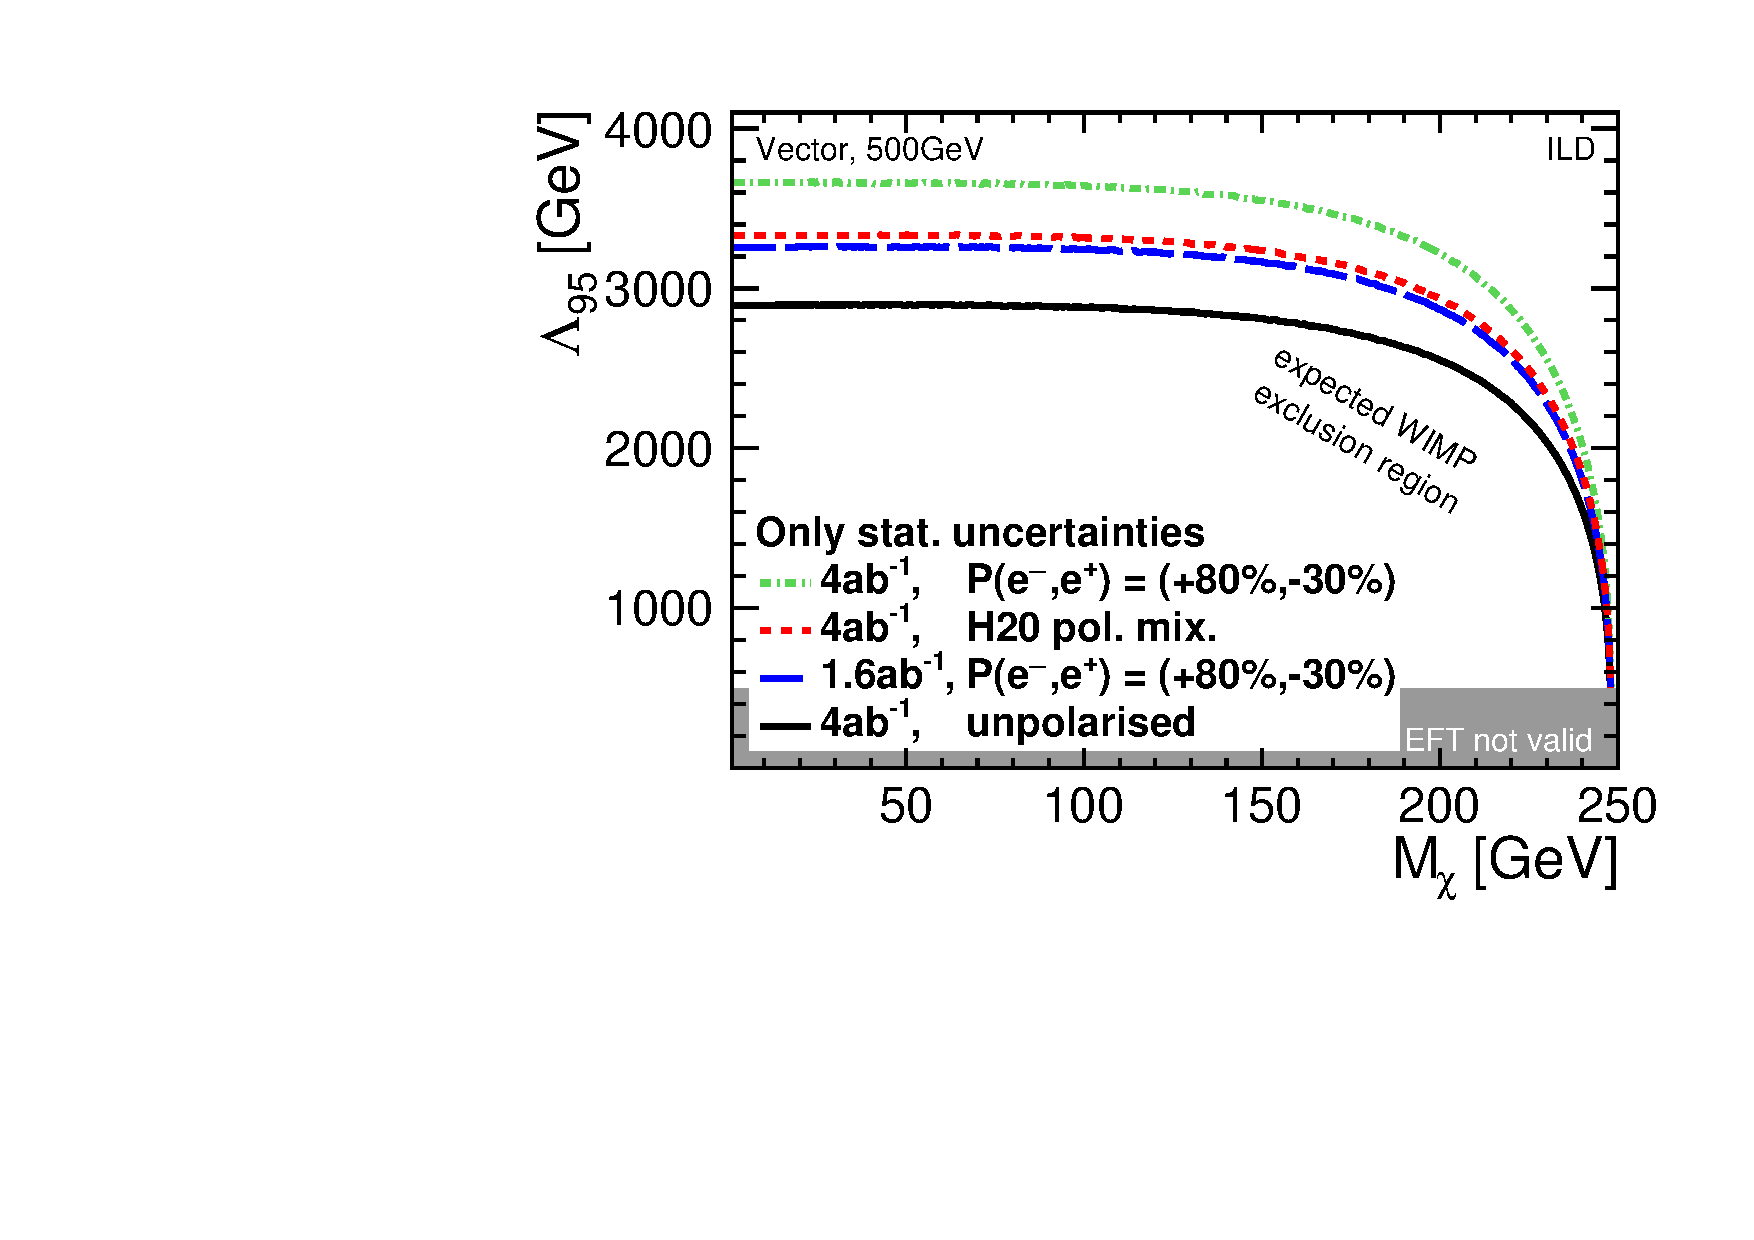
\includegraphics[width=0.95\linewidth]{./chapters/figures/vector_noSystematics.pdf}
		
\caption{Comparison of the reach of the search for WIMP production in the mono-photon channel for different assumptions on luminosity and polarization (see Sec.~\ref{sec:searches} for a description of the analysis)~\cite{Habermehl:417605}. Note that this plot is considering {\em statistical uncertainties only}. The corresponding comparison {\em including systematic uncertainties} is shown in Fig.~\ref{fig:polWIMPsys}.}
\label{fig:polWIMPstat}
\end{figure}

%%%%%%%%%%%%%%%%%%%%%%%%%%%%%%%%%%%%%%%%%%%%%%%%%%%%%%%%%%%%%%%%%%%%%%%%%%%%5

\subsubsection{Analysis of chiral properties} 
\label{subsubsec:pol:chiral}
Beam polarisation is essential to analyze the chiral structure of SM processes in search for deviations from a pure $V-A$ structure due to new physics contributions --- and, in case of a discovery of new particles at the LHC or the ILC itself, of these new particles and their interaction. The list of example applications is long and comprises for instance:
\begin{itemize}
\item Measurements fermion couplings in 2-fermion production: Beam polarisation is essential to disentangle the left- and right-handed couplings of each fermion species to the photon and the $Z$ boson, as discussed in Sec.~\ref{subsec:ew_ffana}. 
\item Measurements of triple gauge couplings: With both beams polarized and using various orientations of the polarisation vectors, all 14 complex couplings (thus 28 real parameters) of the most general Lagrangian for triple gauge vertices, including $CP$ violation, can be extracted simultaneously, as  discussed in Sec.~\ref{subsec:ew_WWana}.
\item Higgs coupling determination: The left-right asymmetry of the $ZH$ cross section has been found to be an important ingredient for constraining the full set of $CP$ conserving dimension-6 operators consistent with $SU(2) \times\ U(1)$ symmetry. This will be discussed in detail in Sec.~\ref{sec:global}.
\item Generic BSM effects: The chiral structure of physics beyond the SM is apriory not known - it could be similar to the SM or completely different. When parametrising new physics in terms of effective operators, the tensor structure of the operator immediately relates to the chiral cross sections: For instance the $s$-channel exchange of a vector mediator allows only for \sigmaLR\ and \sigmaRL\ by angular momentum conservation,
while the exchange of a scalar also has non-zero \sigmaLL\ and \sigmaRR. Since these
vanish in the SM, like-sign polarisation configurations are extremely sensitive to 
such types of new interactions. An example is e.g.\ the distinction between different WIMP models in the mono-photon channel, as discussed in Sec.~\ref{subsec:searches_monophoton}.
\end{itemize}  
% Many more applications can be found e.g.\ in~\cite{MoortgatPick:2005cw, Fujii:2018mli}. 

%%%%%%%%%%%%%%%%%%%%%%%%%%%%%%%%%%%%%%%%%%%%%%%%%%%%%%%%%%%%%%%%%%%%%%%%%%%%5

\subsubsection{Control of systematic uncertainties} 
\label{subsubsec:pol:systematics}

Last but not least, the redundancies provided by the combination of data sets with different beam polarization configurations are invaluable for the control of systematics uncertainties. Thereby it important to always have one more degree of freedom that (statistically) absolutely required: For physics measurements which do not aim at the analysis of a chiral structure, e.g.\ measurements of total unpolarised cross sections, two data sets with with different polarisations (e.g.\ $\Pmp=(\pm 80\%, \mp 30\%)$ or $\Pmp=(\pm 80\%, 0)$ often suffice to constrain the most important nuisance parameters. However if the chiral structure itself is among the observables, e.g.\ when measuring \ALR\ of 2-fermion processes or of Higgsstrahlung, one flip of the polarisation sign(s) is already contained in the observable itself, and thus a non-zero positron polarisation becomes essential to provide enough independent information to constrain nuisance parameters.

The evaluation of systematic uncertainties for experiments which have not yet been built is a difficult task and will to some extent always remain guess-work until real data have been taken. Important is therefore to include the experience from previous $e^+e^-$ experiments, especially at LEP, where many uncertainties could be controled to a typical level of 1\%. Assuming that the same level can be reached at future $e^+e^-$ colliders, detailed studies of systematic uncertainties at the ILC have concentrated on cases where the statistical uncertainties are expected to be significantly below 1\%, and on searches in channels with large irreducible backgrounds. An example for the first case is a global analysis of total rates and differential distributions of various 2-fermion and 4-fermion SM processes, extracting simultaneously the total unpolarised cross sections, the relevant left-right asymmetries, the beam polariations and the charged triple gauge couplings, see Sec.~\ref{subsec:ew_WWana} and Ref.~\cite{bib:PhDRobert}. An example for the second category is the WIMP search in the mono-photon channel, see Sec.~\ref{sec:searches} and Ref.~\cite{Habermehl:417605}. 

In the remainder of this section we will highlight the relative impact of the beam polarisation on the control of systematic uncertainties using these two studies as examples. The consequences for the treatment of systematic uncertainties in the Higgs coupling fit will be discussed in the next subsection.

\begin{itemize}
\item {\textbf{Fast-helicity reversal and correlations between data sets:}} The design of the ILC includes the capability to flip the sign of the two beam polarisations independently and on a train-by-train basis, as introduced in Sec.~\ref{par:beampol}. This helicity reversal is fast compared to typical time-scales of changes in the configuration, calibration and alignment of the detector and the accelerator, and thus data sets with the same beam energy but different beam helicities can be considered as being collected ``quasi-concurrently''. Therefore, many of the experimental systematic effects will be correlated to a large degree between data sets with different polarisations. Note that this does not apply for data sets with different center-of-mass energies, which are collected after each other, typically in different years, and thus systematic effects can in general not be expected to be correlated between such data sets.
Similarly, also most theoretical uncertainties will be correlated between same-energy-different-polarisation data sets, apart from those which directly concern the dependence of the polarised cross sections on the beam polarisations, so effectively any uncertainty to Eqn.~\ref{eq:pol:xsec} {\color{red} [JL: I can't think of any uncertainty to this very basic relation, but I don't dare to say that there is none - comments welcome!]}.  

As example, Fig.~\ref{fig:alpha_error_corr_uncorr} shows the uncertainties $\Delta \alpha $ on the unpolarised cross sections of various 2-fermion and 4-fermion processes as obtained from the global fit introduced above~\cite{bib:PhDRobert}, for the example of a 1\% uncertainty on selection efficiencies and purities, each. In the pesence of beam polarisation, it is assumed that only 10\%, thus 0.1\%, remain uncorrelated between the data sets of different polarisations. In absence of beam polarisation, there are no data sets with correlated systematic uncertainties, and the impact on the cross section uncertainties increases by a factor of 2 for $WW$ and single-$W$ processes, and a factor of 5 for $s$-channel $Z/\gamma$ exchange.
\begin{figure}
\centering
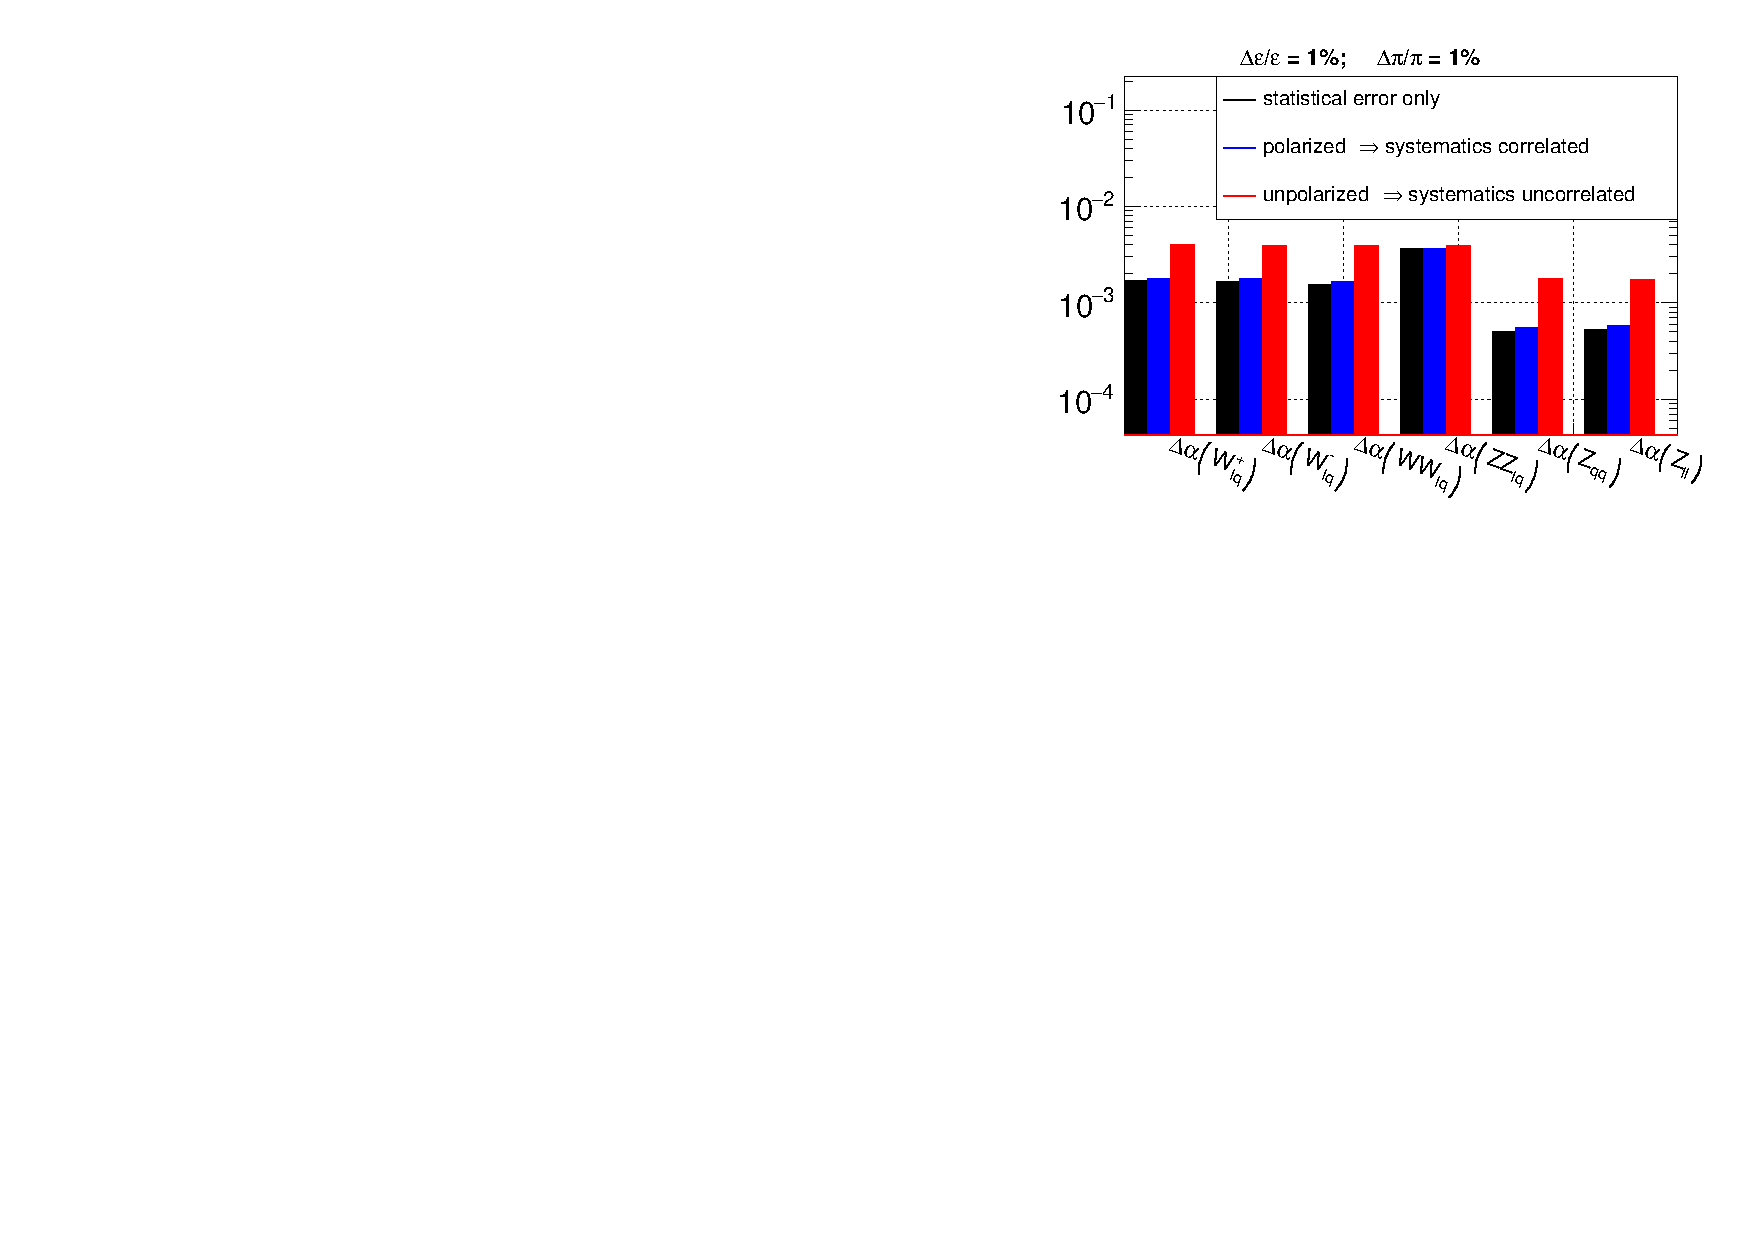
\includegraphics[width=0.95\linewidth]{./chapters/figures/ElectroWeakSysDependency_alpha_short.pdf}
		
\caption{Uncertainties on the unpolarised cross sections of various 2-fermion and 4-fermion processes as obtained from the global fit introduced in the text~\cite{bib:PhDRobert}, assuming a systematic uncertainty of 1\% on the selection efficiencies and purities, each. In the case of polarised beams, it is assumed that only 10\% of the uncertainty is uncorrelated between data sets - in this case the impact of the systematic uncertainties is minimal. Without the redundancies provided by data sets with correlated systematic uncertainties, the total uncertainties increase by a factor 2 for $WW$ and single-$W$ processes and a factor of 5 for 2-fermion processes.}
\label{fig:alpha_error_corr_uncorr}
\end{figure}

Note that this example so far only considers normalisation uncertainties. When adding shape uncertainties, however, the benefit from the redundacy offered by several data sets with correlated systematic effects is expected to be even more pronounced than in the current case of only normalisation uncertainties, since the shape uncertainties will reduce the information which can be extracted from the  differential distributions included in the fit.  

\item {\textbf{Impact of positron polarisation on \ALR\ measurement:}} The left-right asymmetries \ALR\ themselves are obviously only accessible when at least electron beam polarisation is available. Still the positron polarisation is crucial in order to reach ultimate precision on \ALR, as illustrated in Fig.~\ref{fig:beta_error_noposipol}, again from the global fit to 2- and 4-fermion processes. In this example, no detector or theory systematics are included, only the exact polarisation values are treated as nuisance parameters. It can be seen that in the absence of positron polarisation, the uncertainties on \ALR\ increase by 2 factor 2 on $WW$ production and by a factor of $10$ on $s$-channel $Z$ exchange. only the single-$W$ processes remain unaffected.


\begin{figure}
\centering
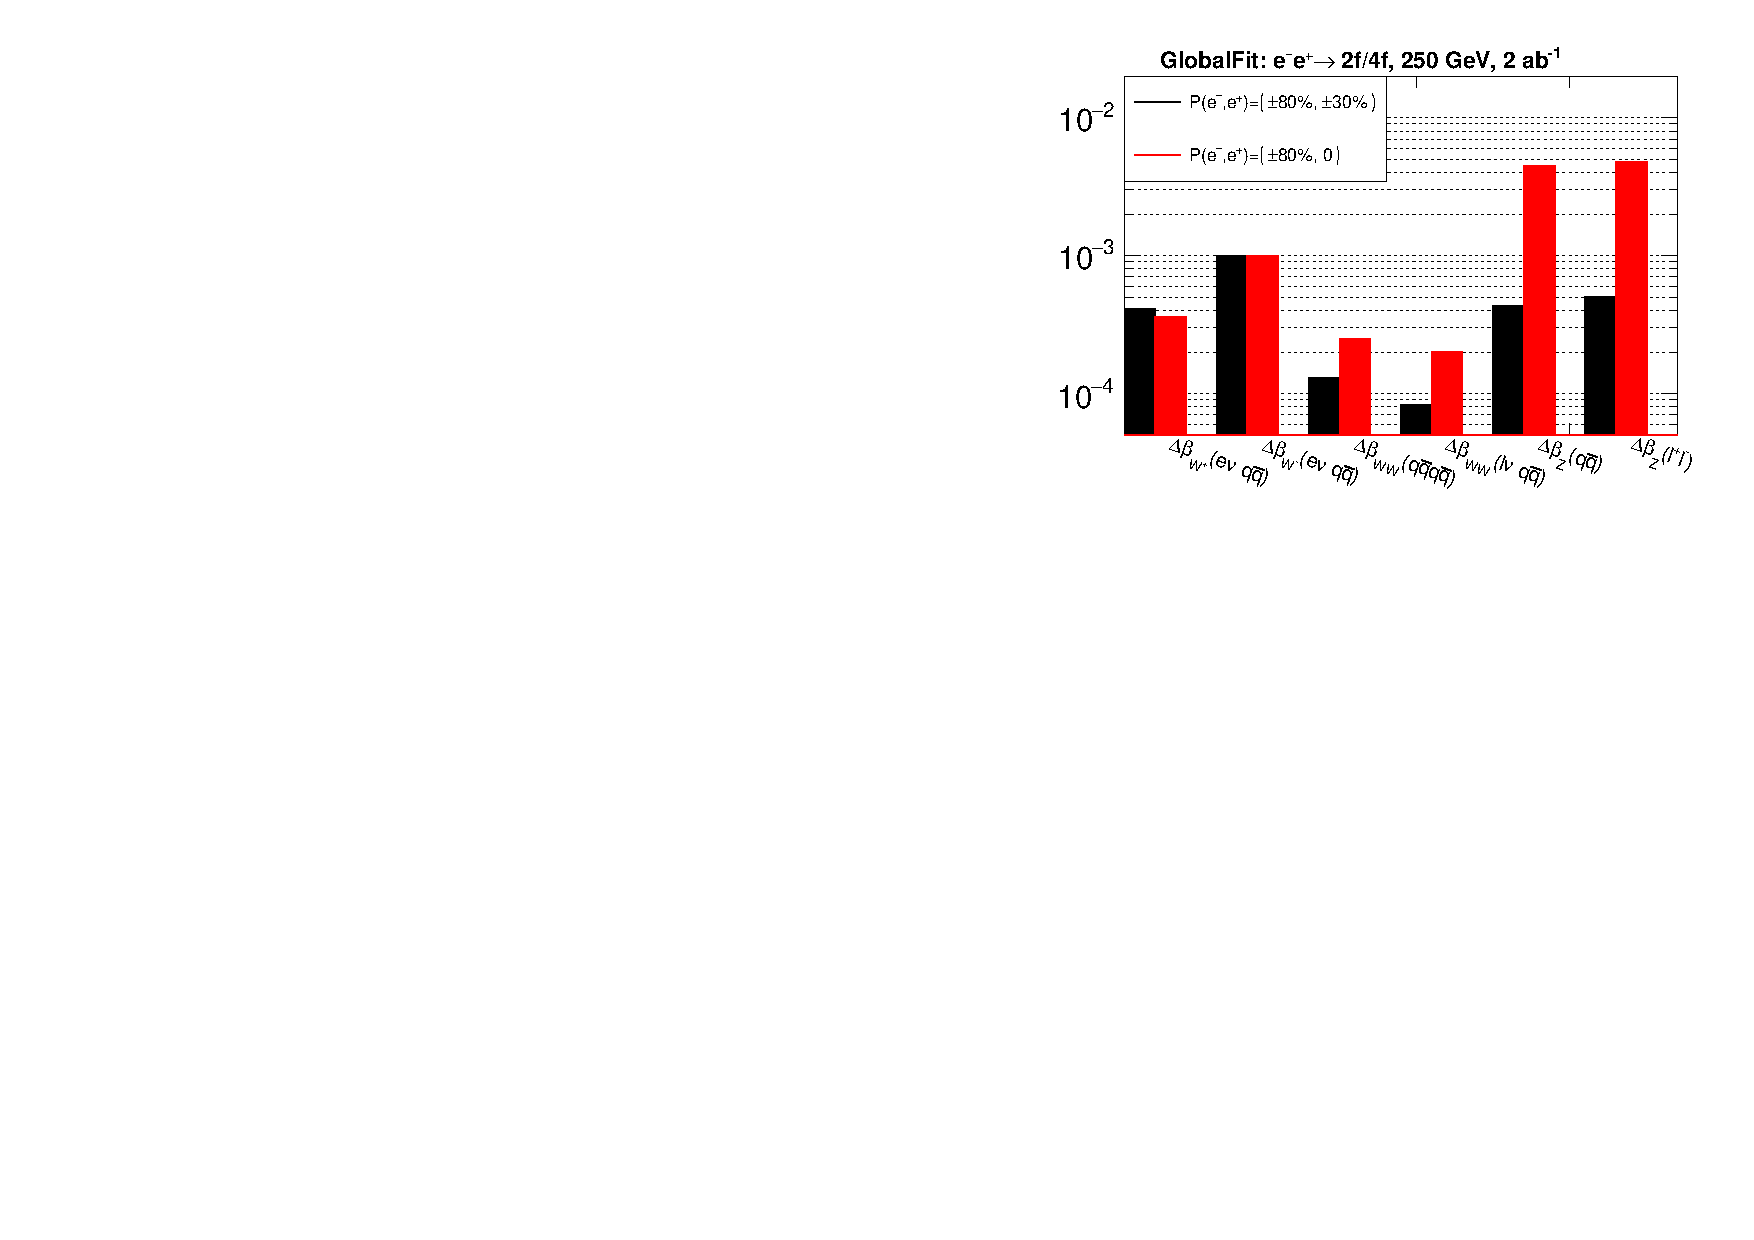
\includegraphics[width=0.95\linewidth]{./chapters/figures/beta_precision_upolarized.pdf}
		
\caption{Uncertainties $\Delta \beta$ on \ALR\ of various 2-fermion and 4-fermion processes as obtained from the global fit introduced in the text~\cite{bib:PhDRobert} with both beams polarised (with the standard 45\%/45\%/5\%/5\% sharing between the four helicity configurations) and in the absence of positron polarisation (with a 50\%/50\% sharing between the two remaining helicity configurations). In the absence of positron polarisation, the  uncertainties on \ALR\ increase by a factor 2 for $WW$ and by about a factor of 10 for 2-fermion processes. Alone the single-$W$ processes remain unaffected.}
\label{fig:beta_error_noposipol}
\end{figure}

\item{\textbf{Undetected biases:}} When considering the level of precision the ILC is aiming for, and even more so when attempting to go even further, even subtle biases can propagate to the results when not treated properly. As example, let's consider the case of operation with an unpolarised positron. In this case, one could assume that it would be fully sufficient to fix the nuisance parameters for the positron polarisation to zero. However it has been shown in~\cite{bib:PhDRobert} that in this case even a residual positron polarisation at the permille-level would already create a noticible bias on cross sections and asymmetries of the same order  of magnitude. This would make it hard to decide whether any possibly observed discrepancy from the SM expectation is a hint for new physics or due to a systematic effect. Therefore for ultimate precision, both beam polarisations should be treated as nuisance parameters independently of their absolute size.

\item {\textbf{Shape uncertainties and beam polarization:}} Uncertainties on the shape of distributions have been included in the WIMP search in the mono-photon channel~\cite{Habermehl:417605}. Figure~\ref{fig:polWIMPsys} shows the expected exclusion limit on the new physics scale $\Lambda$ as function of the WIMP mass for the same study cases as Fig.~\ref{fig:polWIMPstat}. The study includes a careful evaluation of the systematic uncertainties, comprising those on selection efficiencies, luminosity, beam energy (spectrum) and polarization as well as on the theoretical modelling of the background. 
The limit calculation uses a fractional event counting based on the observed energy spectrum of the selected photon candidates and considers normalisation and shape-dependent uncertainties as well as their (partial) correpations. The signal strength thereby has to be constrained on top of a significant irreducible background from $e^+e^- \to \nu\bar{\nu}\gamma$ and radiative low-angle Bhabha scattering. For increasing WIMP masses, the maximum possible energy of the ISR photons becomes lower. For the highest WIMP masses, the signal-free part of the spectrum becomes sufficiently large to constrain the nuisance parameters and thus to limited the impact of the systematic uncertainties. This effect is visible in form of the ``bump'' in the limit curves near $M_X=220$\,GeV. In case of the unpolarised data set, the effect starts to become visible already from $M_X=150$\,GeV onwards,
but the exclusion remains much weaker than in the polarised case. Comparison with Fig.~\ref{fig:polWIMPstat} shows that the benefit of polarisation in presence of systematic uncertainties goes significantly beyond the purely statistical $S/B$ effect. In particular it should be noted that when the systematic effects are included, the splitting of the total luminosity into four different data sets allows to set more stringent limits as if all luminosity would just be dedicated to the ``statistically-prefered'' helicity combination. In fact the result for only one helicity combination suffers as much from the systematic uncertainties as the unpolarised case, while in case of the polarisation mix, when four data sets with different helicities are used, the sensitivity is only affected veru weakly by the systematic uncertainties.



\begin{figure}
\centering
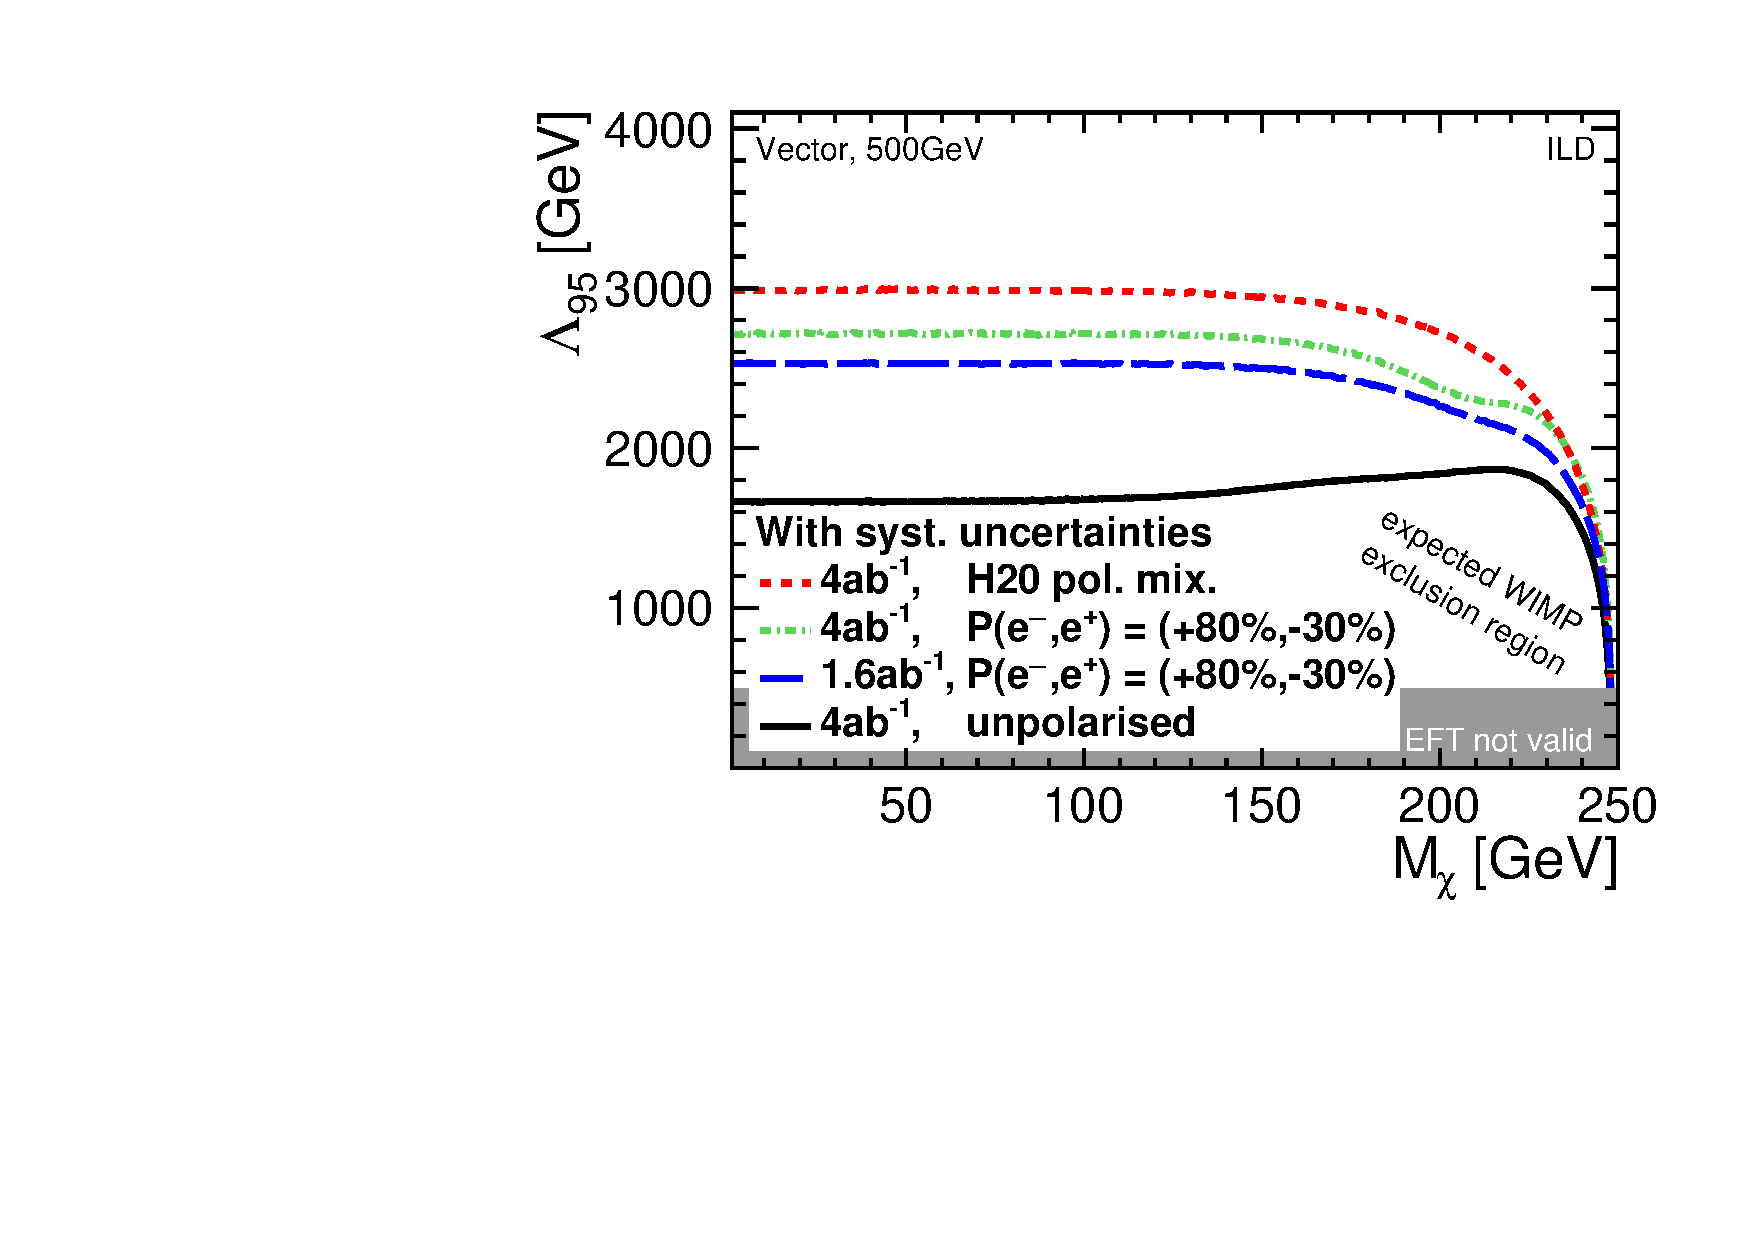
\includegraphics[width=0.95\linewidth]{./chapters/figures/vector_withSystematics.pdf}
		
\caption{Comparison of the reach of the search for WIMP production in the mono-photon channel for different assumptions on luminosity and polarization, {\em including} systematic uncertainties (see Sec.~\ref{sec:searches} for a description of the analysis)~\cite{Habermehl:417605}. }
\label{fig:polWIMPsys}
\end{figure}

\end{itemize}

\subsubsection{Systematic uncertainties considered in the Higgs coupling fit}
The Higgs coupling fits discussed in the following sections include the following systematic uncertainties:
\begin{itemize}
\item The luminosity at the ILC will be measured from low-angle Bhabha scattering with the help of a dedicated forward calorimeters, the LumiCals (see Sec.~\ref{sec:detectors} and Ref.~\cite{Abramowicz:2010bg}). This measurement is extremely sensitive to the exact alignment of the LumiCals on the two sides of the detector, as well as to beam backgrounds and has been studied in detailed simulations both for the ILC and for CLIC~\cite{Bozovic-Jelisavcic:2014aza, Lukic:2013fw}. Based on these studies, the resulting systematic uncertainty on all Higgs cross section and cross-section-times-braching-ratio measurements is assumed to be 0.1\%
\item Another 0.1\% is assumed for the net systematic effect of the finite knowledge of luminosity-weighted long-term average values of the beam polarisations at the $e^+e^-$ interaction point. While the Compton polarimeters in the Beam Delivery System resolve time-dependencies at the level of 0.25\%~\cite{Vormwald:2015hla, List:2015lsa}, also the effects of spin transport, misalignment of beam line magnets as well as depolarisation during the beam-beam interaction have been studied~\cite{Beckmann:2014mka}. The absolute scale of the luminosity-weighted average polarisation at the IP is finally calibrated from collision data, e.g.\ a global fit SM processes with a strong polarisation dependence~\cite{bib:PhDRobert}. 
\item Theoretical uncertainties are also assumed to have reched at the level of 0.1\% by the time of ILC operation {\color{red}[Any good \textbf{theoretical} arguments to add here?]}. This number is justified in case of polarised beams by the global fit study discussed above~\cite{bib:PhDRobert}, which showed that the absolute normalisations of cross sections and left-right asymetries can be controled  at this level. In the case of unpolarised beams, the theoretical uncertainties would require a much more detailed consideration.
\item As mentioned already at the beginning of Sec.~\ref{subsubsec:pol:systematics} experimental systematics on selection efficiencies, flavour tagging, detector calibrations etc of 1\% have already been reached at LEP in many cases. With the advances in detector technology and the larger integrated luminosity, we assume that for each data set at the ILC this can be reduced by a factor of 3 to 0.3\%. These 0.3\% are considered as net effect of all experimental uncertainties in the absence of beam polarisation.

In the presence of both beam polarisations, the net effect of systematic uncertainties has been shown to be smaller by factors between 2 and 10 due to the correlations between data sets with different beam polarisations as discussed in Sec.~\ref{subsubsec:pol:systematics}. Since the Higgs coupling fit does not yet comprise such a detailed treatment of systematic uncertainties and their correlations as the above mentioned global fit to 2-fermion and 4-fermion processes, we assume that, in presence of polarised beams, the net effect of the experimental uncertainties reduces to 0.1\%.
\end{itemize}


%%%%%%%% to be moved to IX C %%%%%%%%%%%%%%%%%%%%%%%%%%%%%

{\color{red}[THE FOLLOWING IS TO BE MOVED TO SECTION~\ref{subsec:lincirc}]}\\
Figure~\ref{fig:polWIMPmanhattans} shows the 95\% CL reach in new physics scale $\Lambda$ for pair production of a light ($M_{X} = 1$\,GeV) WIMP mediated by a vector operator for different assumptions on luminosity, energy and polarization 
as they are typical for linear and circular colliders. In particular the polarised
configurations al refer to the ILC reference running scenario H20, see Sec.~\ref{sec:runscenarios}. Input to the limit calculation is the ILC study performed in full detector simulation of the ILD detector concept described in~Sec.~\ref{sec:searches}, and its extrapolation to other center-of-mass energies~\cite{Habermehl:417605}. The study includes a careful evaluation of the systematic uncertainties, comprising those on selection efficiencies, luminosity, beam energy (spectrum) and polarization as well as on the theoretical modelling of the background. The limit calculation uses a fractional event counting based on the 
energy spectrum of the photon. It can be seen that at 250\,GeV, 2\,\iab\ with polarized beams offer a greater reach than 5 or even 10\,\iab\ without beam polarization. Even at a higher center-of-mass energy of 350\,GeV, about 10\,\iab\ of unpolarised data  would be required to catch up with 2\,\iab\ of polarised data at 250\,GeV. The higher center-of-mass energies reachable by linear colliders, in conjuction with beam polarisation, improve the reach considerably. For instance the reach of the full H20 running scenario of the ILC roughly doubles the reach in $\Lambda$ compared to the 250\,GeV stage.

\begin{figure}
\centering
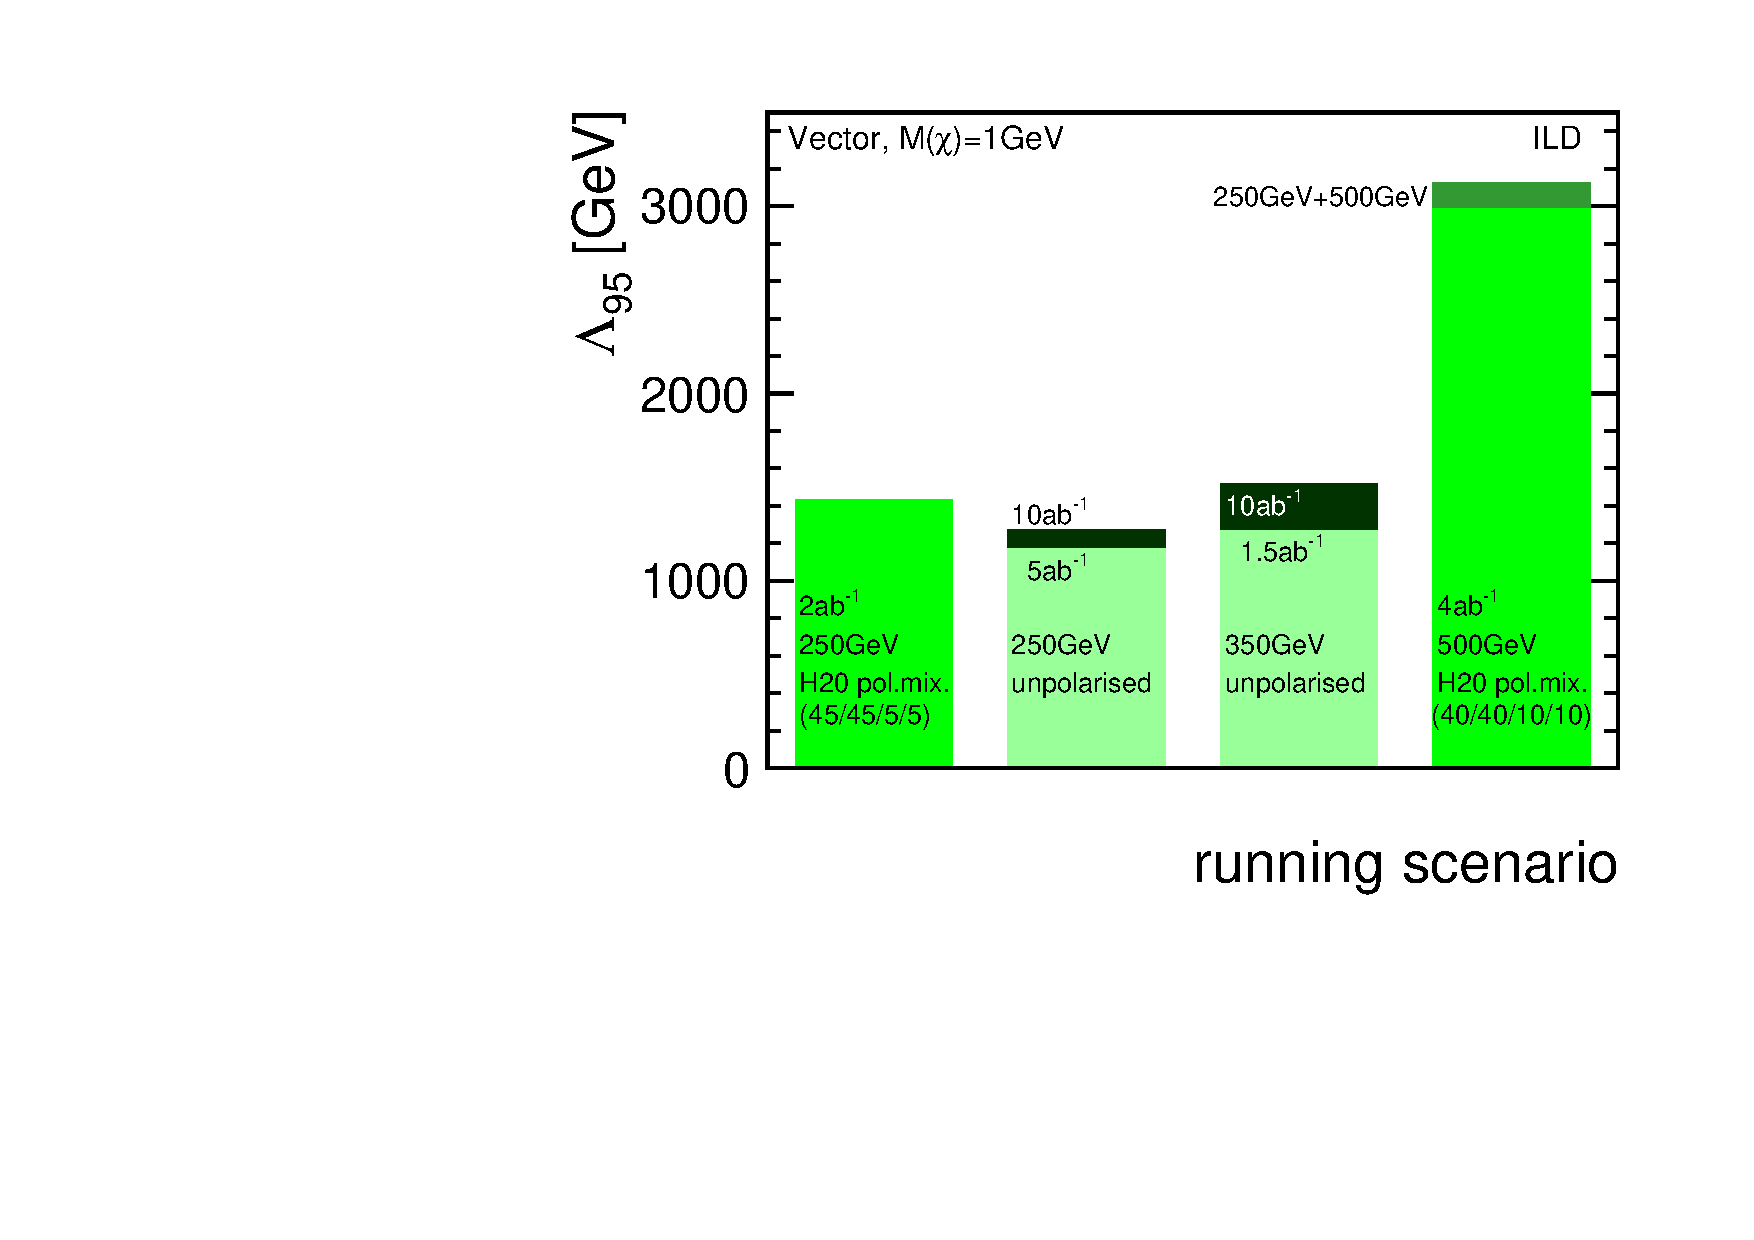
\includegraphics[width=0.95\linewidth]{./chapters/figures/manhattan_vector_v3.pdf}
		
\caption{{\color{red}[Michael, I think this plot and its description would better fit into section~\ref{subsec:lincirc}, but I didn't want to mess with `your' tex file. Please move it to your section if you like!]} Comparison of the reach for WIMP searches in the mono-photon channel for different assumptions on luminosity, polarization and energy, including systematic uncertainties (see Sec.~\ref{sec:searches} for a description of the analysis)~\cite{Habermehl:417605}. }
\label{fig:polWIMPmanhattans}
\end{figure}






Beam polarization is considered as an essential ingredient of the ILC physics program because of three important advantages:
\begin{enumerate}
\item Suppression of backgrounds and enhancement of signals
\item Analysis of the chiral properties
\item Control of systematic uncertainties
\end{enumerate}
The first two items often (but not always!) apply to a large extent already when only electron polarisation is available. 
However for the third aspect, the positron polarisation is crucial in many cases --- in particular whenever the left-right asymmetry \ALR\ itself is the physics observable, like \eg\ for 2-fermion processes (see Sec.~\ref{subsec:ew_ffana}) or for the Higgs precision measurements (see Sec.~\ref{subsec:ew_WWana}).
All three aspects will be discussed and illustrated with concrete physics examples in the following subsections. 

A comprehensive review of the role of polarization with many more examples can be found in~\cite{MoortgatPick:2005cw}, and a recent discussion of positron polarization in particular in~\cite{Fujii:2018mli}. 

%%%%%%%%%%%%%%%%%%%%%%%%%%%%%%%%%%%%%%%%%%%%%%%%%%%%%%%%%%%%%%%%%%%%%%%%%%%%5

\subsubsection{Suppression of backgrounds and enhancement of signals} 
\label{subsubsec:pol:s_over_b}
Due to the chiral structure of the weak interaction, and especially since right-handed fermions form isospin-singlets and therefore don't participate in charged current interactions, every $e^+e^-$ cross section depends on the chirality of the incoming beam particles.  For any given polarization of the electron and positron beams, \Pem\ and \Pep, respectively, the polarised cross section is caluculated from the chiral cross sections in the following way:
\begin{eqnarray}
\sigma_{\Pem\Pep} &=& \frac{1}{4}\bigl\{
     (1+\Pem)(1+\Pep) \quad \sigmaRR  \nonumber \\
&& + (1-\Pem)(1-\Pep) \sigmaLL \nonumber \\
&& + (1+\Pem)(1-\Pep) \sigmaRL \nonumber \\ 
&& + (1-\Pem)(1+\Pep) \sigmaLR \bigr\},
\label{eq:pol:xsec}
\end{eqnarray}


For charged current $t$-channel processes, like $e^+e^- \to W^+W^-$, $e^+e^- \to \nu_e\bar{\nu}_e$ or Higgs production via $WW$ fusion, only the \sigmaLR\ contribution is allowed, so that their rate can be dialed up or down by a factor 17 for $\Pmp=(\pm 80\%,\mp 30\%)$ (36 for $\Pmp=(\pm 80\%,\mp 60\%)$) via the choice of the polarisation sign. 

For $s$-channel processes in the SM, including Higgsstrahlung, \sigmaLR\ and \sigmaRL\ contribute. In this case, Eqn~\ref{eq:pol:xsec} can be reduced to
\begin{equation}
 \sigma_{\Pem\Pep} = 2 \sigma_0 (\Leff/\mathcal{L}) \left[1 - \ALR \Peff \right]
\label{eq:pol:xsecschan}
\end{equation}
Here, $\sigma_0$ is the unpolarized cross section and \ALR\ 
the left-right asymmetry, defined in Eqn.~\ref{eq:defALR}. \Leff\ and \Peff\  
are the effective luminosity and polarization, respectively, defined as
\begin{equation}
\Peff= \frac{\Pem - \Pep}{1 - \Pep\Pem}
\label{eq:def-leff-peff}
\quad\mbox{\rm and }\quad
\Leff=\frac{1}{2}(1 -\Pep\Pem)\L
\end{equation}

In practice, for $\Pmp=(\pm 80\%,\mp 30\%)$, $\Peff = \pm 89\%$ and $\Leff = 62\% \mathcal{L}$, whereas for $\Pmp=(0,0)$ and , $\Peff = 0$ and $\Leff = 50\% \mathcal{L}$, since in half of the cases a left-handed electron will meet a left-handed positron --- for which the cross section for $s$-channel processes is zero. 

With \ALR = 0.151 for Higgsstrahlung, this means that the cross section for $\Pmp=(-80\%,+30\%)$ is 41\% larger than the unpolarised cross section, while it is
still 7\% larger than the unpolarised cross section for the opposite sign combination  $\Pmp=(+80\%,-30\%)$. Since, as we saw above, important background processes like $e^+e^- \to W^+W^-$ are strongly suppressed in this configuration, the $\Pmp=(+80\%,-30\%)$ gives comparable and in some cases even better results than the $\Pmp=(-80\%,+30\%)$ configuration. 

However the signal-to-background ratio ($S/B$ or $S/sqrt{B}$) cannot be maximized for all processes at the same time. But it is very important to realize that the combination of a high-$S/B$ data set with a low-$S/B$ data set is statistically {\em not} equivalent to taking 
the same amount of data with the average $S/B$, simply because significances don't add up linearly. Therefore the overall precision increases even if the total intergrated luminosity is split between ``optimal'' and ``non-optimal'' configurations. 

This is illustrated in Fig.~\ref{fig:polWIMPstat}, which compares the reach of the search for WIMP production in the mono-photon channel for different assumptions on luminosity and polarization (see Sec.~\ref{sec:searches} for a description of the analysis). It clearly shows the large increase in sensitivity for \Pmp=(+80\%, -30\%) w.r.t.\ the unpolarised case, and that the result for splitting the data on all four helicity configurations as forseen in the H20 running scenario, albeit completely dominated by the 1.6\,\iab\ collected with \Pmp=(+80\%, -30\%), is still probing significantly higher scales than the unpolarised case. Note that this figure omits all systematic uncertainties in order to highlight the statistical $S/B$ effect. 
\begin{figure}
\centering
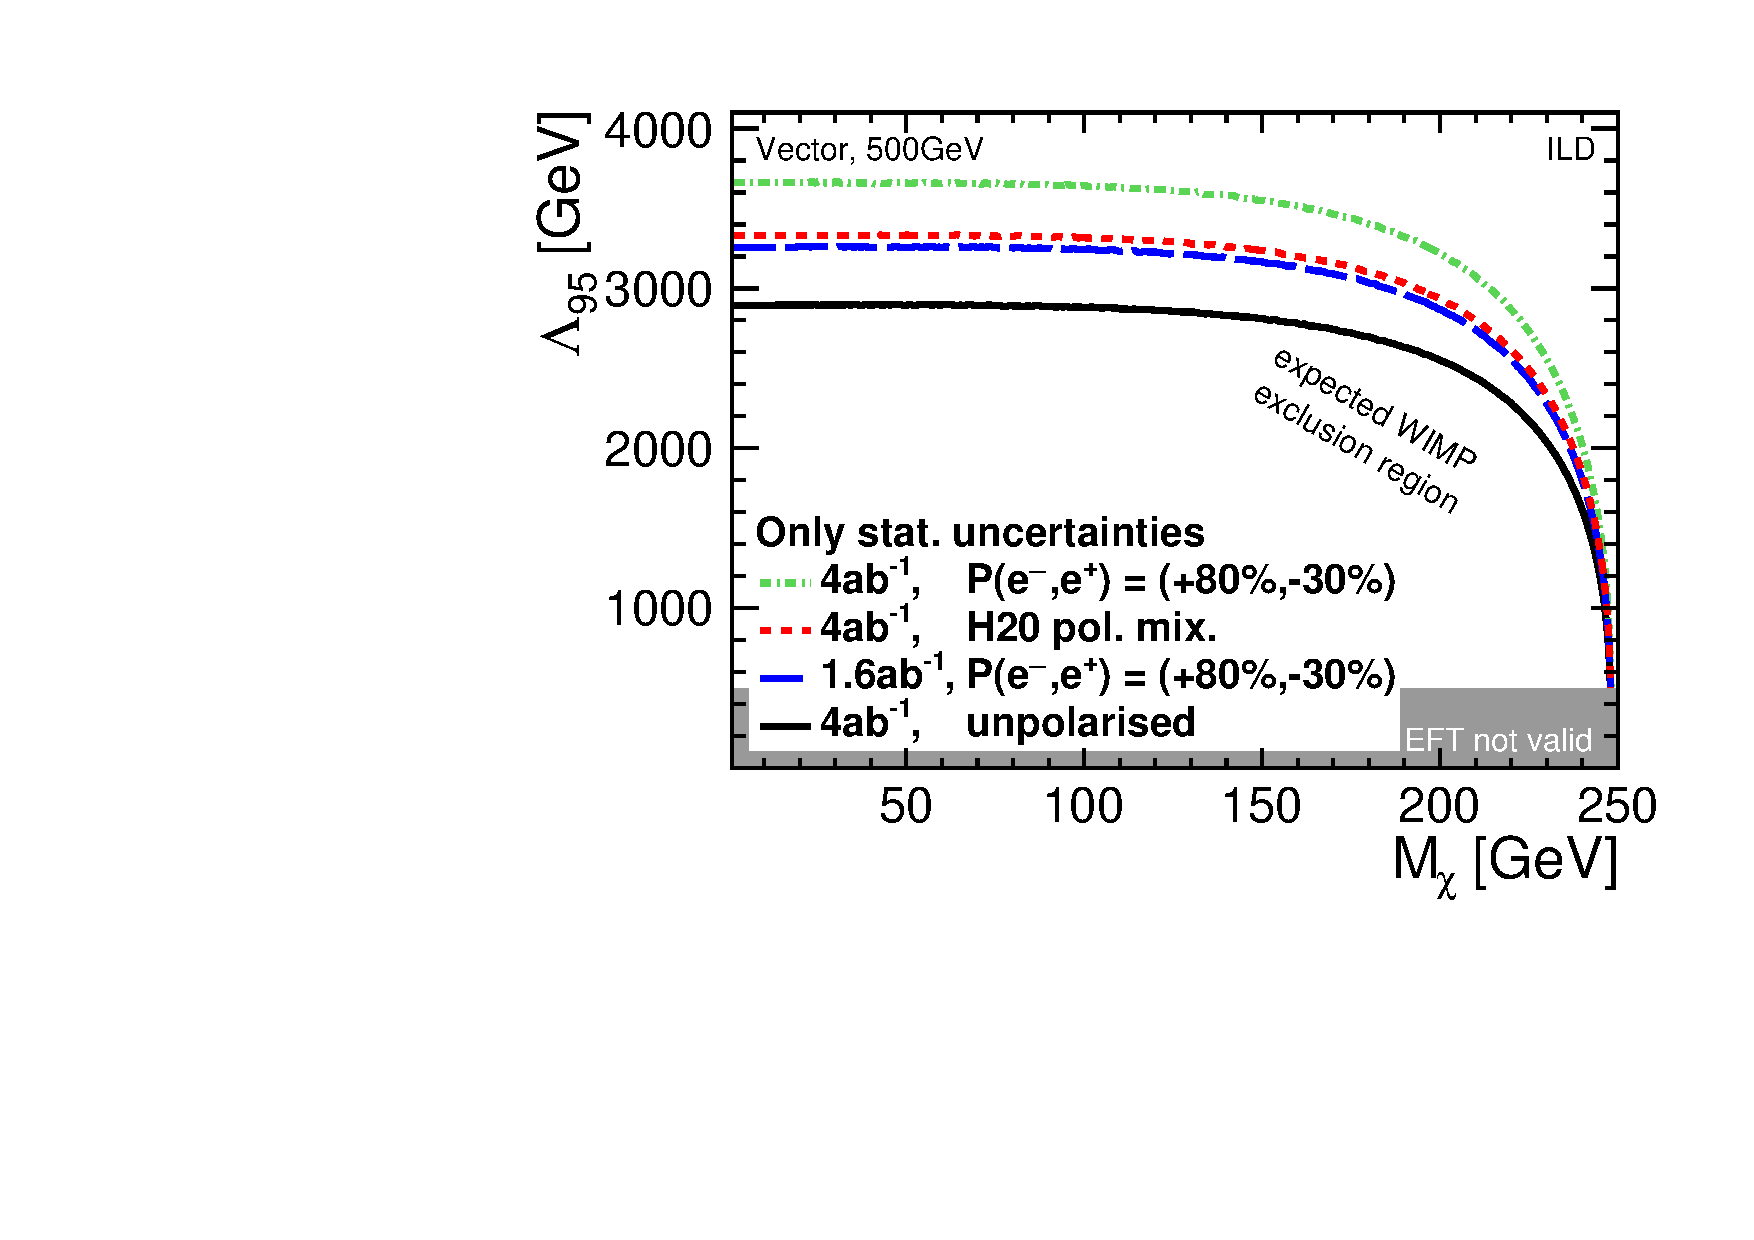
\includegraphics[width=0.95\linewidth]{./chapters/figures/vector_noSystematics.pdf}
		
\caption{Comparison of the reach of the search for WIMP production in the mono-photon channel for different assumptions on luminosity and polarization (see Sec.~\ref{sec:searches} for a description of the analysis)~\cite{Habermehl:417605}. Note that this plot is considering {\em statistical uncertainties only}. The corresponding comparison {\em including systematic uncertainties} is shown in Fig.~\ref{fig:polWIMPsys}.}
\label{fig:polWIMPstat}
\end{figure}

%%%%%%%%%%%%%%%%%%%%%%%%%%%%%%%%%%%%%%%%%%%%%%%%%%%%%%%%%%%%%%%%%%%%%%%%%%%%5

\subsubsection{Analysis of chiral properties} 
\label{subsubsec:pol:chiral}
Beam polarisation is essential to analyze the chiral structure of SM processes in search for deviations from a pure $V-A$ structure due to new physics contributions --- and, in case of a discovery of new particles at the LHC or the ILC itself, of these new particles and their interaction. The list of example applications is long and comprises for instance:
\begin{itemize}
\item Measurements fermion couplings in 2-fermion production: Beam polarisation is essential to disentangle the left- and right-handed couplings of each fermion species to the photon and the $Z$ boson, as discussed in Sec.~\ref{subsec:ew_ffana}. 
\item Measurements of triple gauge couplings: With both beams polarized and using various orientations of the polarisation vectors, all 14 complex couplings (thus 28 real parameters) of the most general Lagrangian for triple gauge vertices, including $CP$ violation, can be extracted simultaneously, as  discussed in Sec.~\ref{subsec:ew_WWana}.
\item Higgs coupling determination: The left-right asymmetry of the $ZH$ cross section has been found to be an important ingredient for constraining the full set of $CP$ conserving dimension-6 operators consistent with $SU(2) \times\ U(1)$ symmetry. This will be discussed in detail in Sec.~\ref{sec:global}.
\item Generic BSM effects: The chiral structure of physics beyond the SM is apriory not known - it could be similar to the SM or completely different. When parametrising new physics in terms of effective operators, the tensor structure of the operator immediately relates to the chiral cross sections: For instance the $s$-channel exchange of a vector mediator allows only for \sigmaLR\ and \sigmaRL\ by angular momentum conservation,
while the exchange of a scalar also has non-zero \sigmaLL\ and \sigmaRR. Since these
vanish in the SM, like-sign polarisation configurations are extremely sensitive to 
such types of new interactions. An example is e.g.\ the distinction between different WIMP models in the mono-photon channel, as discussed in Sec.~\ref{subsec:searches_monophoton}.
\end{itemize}  
% Many more applications can be found e.g.\ in~\cite{MoortgatPick:2005cw, Fujii:2018mli}. 

%%%%%%%%%%%%%%%%%%%%%%%%%%%%%%%%%%%%%%%%%%%%%%%%%%%%%%%%%%%%%%%%%%%%%%%%%%%%5

\subsubsection{Control of systematic uncertainties} 
\label{subsubsec:pol:systematics}

Last but not least, the redundancies provided by the combination of data sets with different beam polarization configurations are invaluable for the control of systematics uncertainties. Thereby it important to always have one more degree of freedom that (statistically) absolutely required: For physics measurements which do not aim at the analysis of a chiral structure, e.g.\ measurements of total unpolarised cross sections, two data sets with with different polarisations (e.g.\ $\Pmp=(\pm 80\%, \mp 30\%)$ or $\Pmp=(\pm 80\%, 0)$ often suffice to constrain the most important nuisance parameters. However if the chiral structure itself is among the observables, e.g.\ when measuring \ALR\ of 2-fermion processes or of Higgsstrahlung, one flip of the polarisation sign(s) is already contained in the observable itself, and thus a non-zero positron polarisation becomes essential to provide enough independent information to constrain nuisance parameters.

The evaluation of systematic uncertainties for experiments which have not yet been built is a difficult task and will to some extent always remain guess-work until real data have been taken. Important is therefore to include the experience from previous $e^+e^-$ experiments, especially at LEP, where many uncertainties could be controled to a typical level of 1\%. Assuming that the same level can be reached at future $e^+e^-$ colliders, detailed studies of systematic uncertainties at the ILC have concentrated on cases where the statistical uncertainties are expected to be significantly below 1\%, and on searches in channels with large irreducible backgrounds. An example for the first case is a global analysis of total rates and differential distributions of various 2-fermion and 4-fermion SM processes, extracting simultaneously the total unpolarised cross sections, the relevant left-right asymmetries, the beam polariations and the charged triple gauge couplings, see Sec.~\ref{subsec:ew_WWana} and Ref.~\cite{bib:PhDRobert}. An example for the second category is the WIMP search in the mono-photon channel, see Sec.~\ref{sec:searches} and Ref.~\cite{Habermehl:417605}. 

In the remainder of this section we will highlight the relative impact of the beam polarisation on the control of systematic uncertainties using these two studies as examples. The consequences for the treatment of systematic uncertainties in the Higgs coupling fit will be discussed in the next subsection.

\begin{itemize}
\item {\textbf{Fast-helicity reversal and correlations between data sets:}} The design of the ILC includes the capability to flip the sign of the two beam polarisations independently and on a train-by-train basis, as introduced in Sec.~\ref{par:beampol}. This helicity reversal is fast compared to typical time-scales of changes in the configuration, calibration and alignment of the detector and the accelerator, and thus data sets with the same beam energy but different beam helicities can be considered as being collected ``quasi-concurrently''. Therefore, many of the experimental systematic effects will be correlated to a large degree between data sets with different polarisations. Note that this does not apply for data sets with different center-of-mass energies, which are collected after each other, typically in different years, and thus systematic effects can in general not be expected to be correlated between such data sets.
Similarly, also most theoretical uncertainties will be correlated between same-energy-different-polarisation data sets, apart from those which directly concern the dependence of the polarised cross sections on the beam polarisations, so effectively any uncertainty to Eqn.~\ref{eq:pol:xsec} {\color{red} [JL: I can't think of any uncertainty to this very basic relation, but I don't dare to say that there is none - comments welcome!]}.  

As example, Fig.~\ref{fig:alpha_error_corr_uncorr} shows the uncertainties $\Delta \alpha $ on the unpolarised cross sections of various 2-fermion and 4-fermion processes as obtained from the global fit introduced above~\cite{bib:PhDRobert}, for the example of a 1\% uncertainty on selection efficiencies and purities, each. In the pesence of beam polarisation, it is assumed that only 10\%, thus 0.1\%, remain uncorrelated between the data sets of different polarisations. In absence of beam polarisation, there are no data sets with correlated systematic uncertainties, and the impact on the cross section uncertainties increases by a factor of 2 for $WW$ and single-$W$ processes, and a factor of 5 for $s$-channel $Z/\gamma$ exchange.
\begin{figure}
\centering
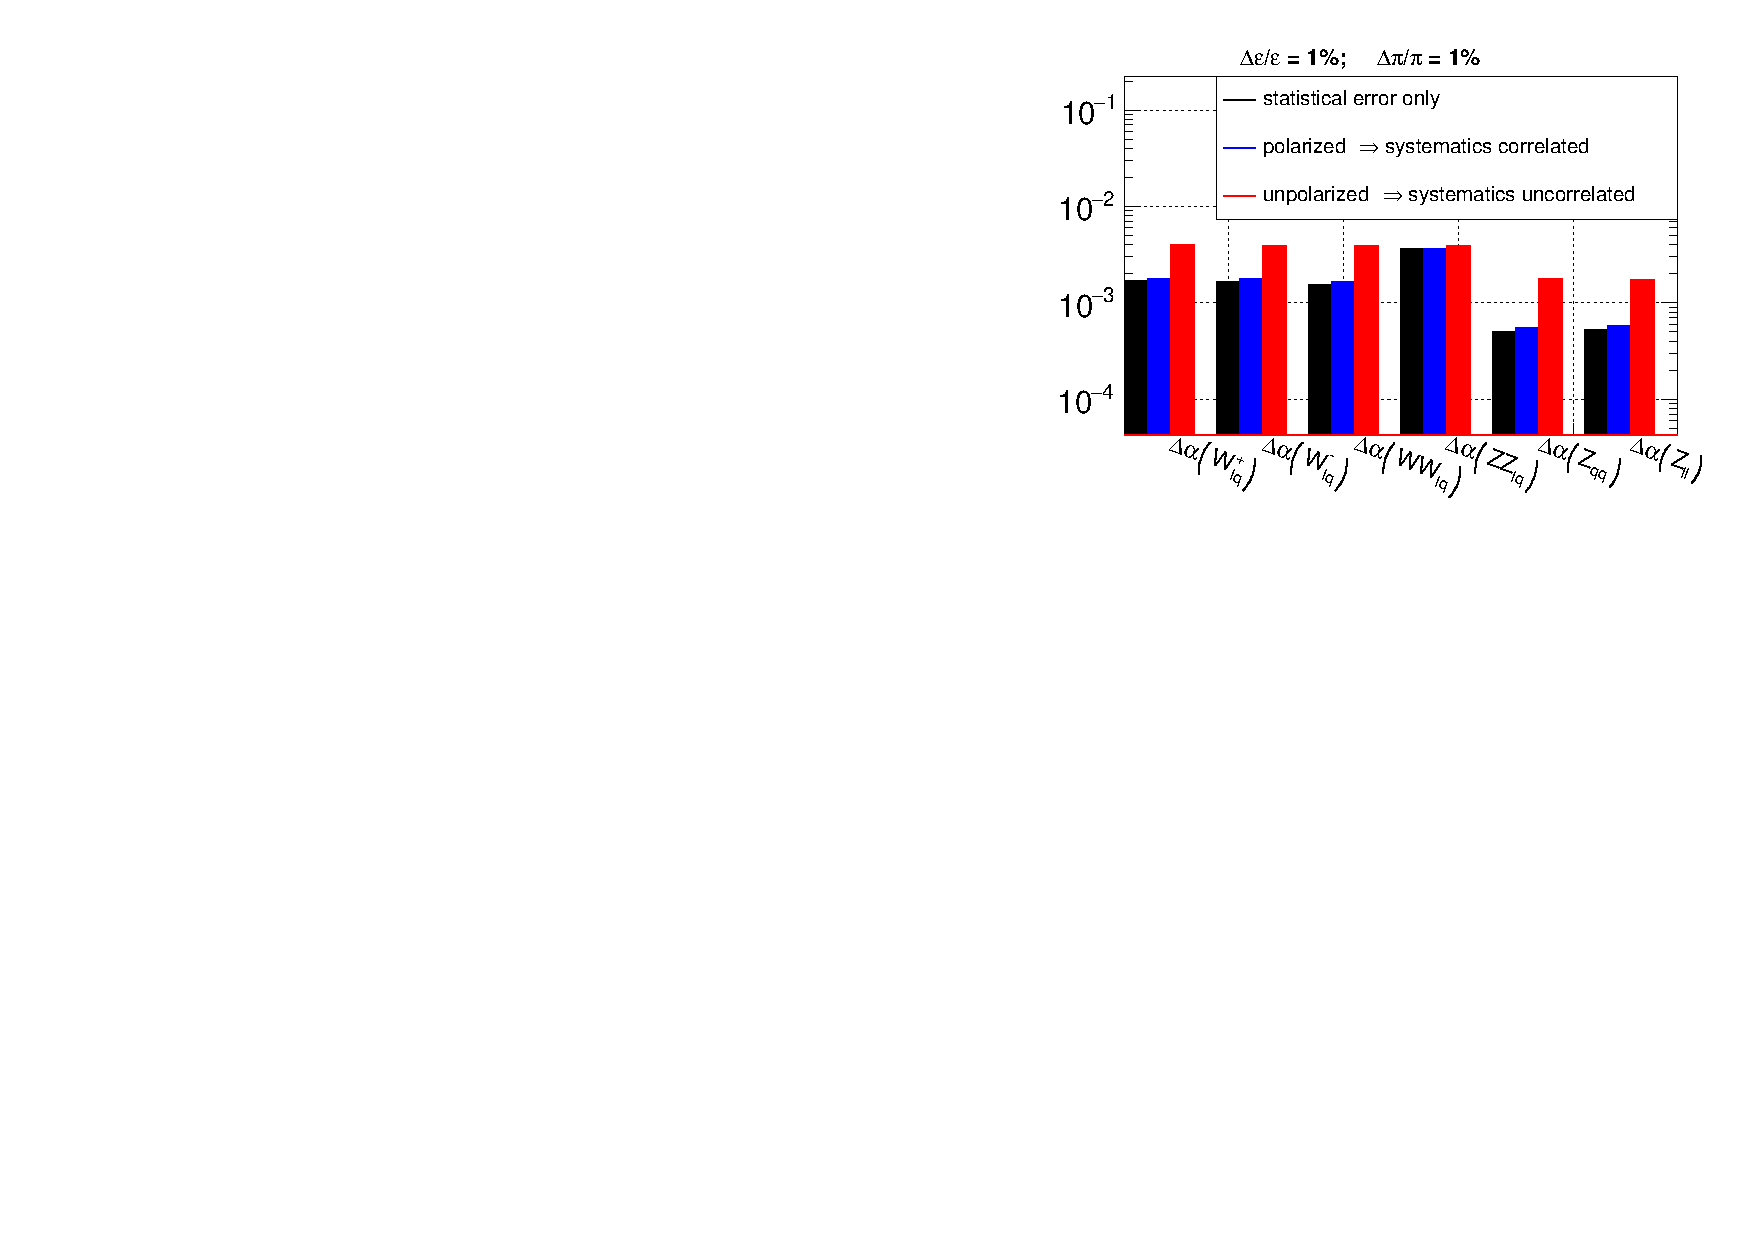
\includegraphics[width=0.95\linewidth]{./chapters/figures/ElectroWeakSysDependency_alpha_short.pdf}
		
\caption{Uncertainties on the unpolarised cross sections of various 2-fermion and 4-fermion processes as obtained from the global fit introduced in the text~\cite{bib:PhDRobert}, assuming a systematic uncertainty of 1\% on the selection efficiencies and purities, each. In the case of polarised beams, it is assumed that only 10\% of the uncertainty is uncorrelated between data sets - in this case the impact of the systematic uncertainties is minimal. Without the redundancies provided by data sets with correlated systematic uncertainties, the total uncertainties increase by a factor 2 for $WW$ and single-$W$ processes and a factor of 5 for 2-fermion processes.}
\label{fig:alpha_error_corr_uncorr}
\end{figure}

Note that this example so far only considers normalisation uncertainties. When adding shape uncertainties, however, the benefit from the redundacy offered by several data sets with correlated systematic effects is expected to be even more pronounced than in the current case of only normalisation uncertainties, since the shape uncertainties will reduce the information which can be extracted from the  differential distributions included in the fit.  

\item {\textbf{Impact of positron polarisation on \ALR\ measurement:}} The left-right asymmetries \ALR\ themselves are obviously only accessible when at least electron beam polarisation is available. Still the positron polarisation is crucial in order to reach ultimate precision on \ALR, as illustrated in Fig.~\ref{fig:beta_error_noposipol}, again from the global fit to 2- and 4-fermion processes. In this example, no detector or theory systematics are included, only the exact polarisation values are treated as nuisance parameters. It can be seen that in the absence of positron polarisation, the uncertainties on \ALR\ increase by 2 factor 2 on $WW$ production and by a factor of $10$ on $s$-channel $Z$ exchange. only the single-$W$ processes remain unaffected.


\begin{figure}
\centering
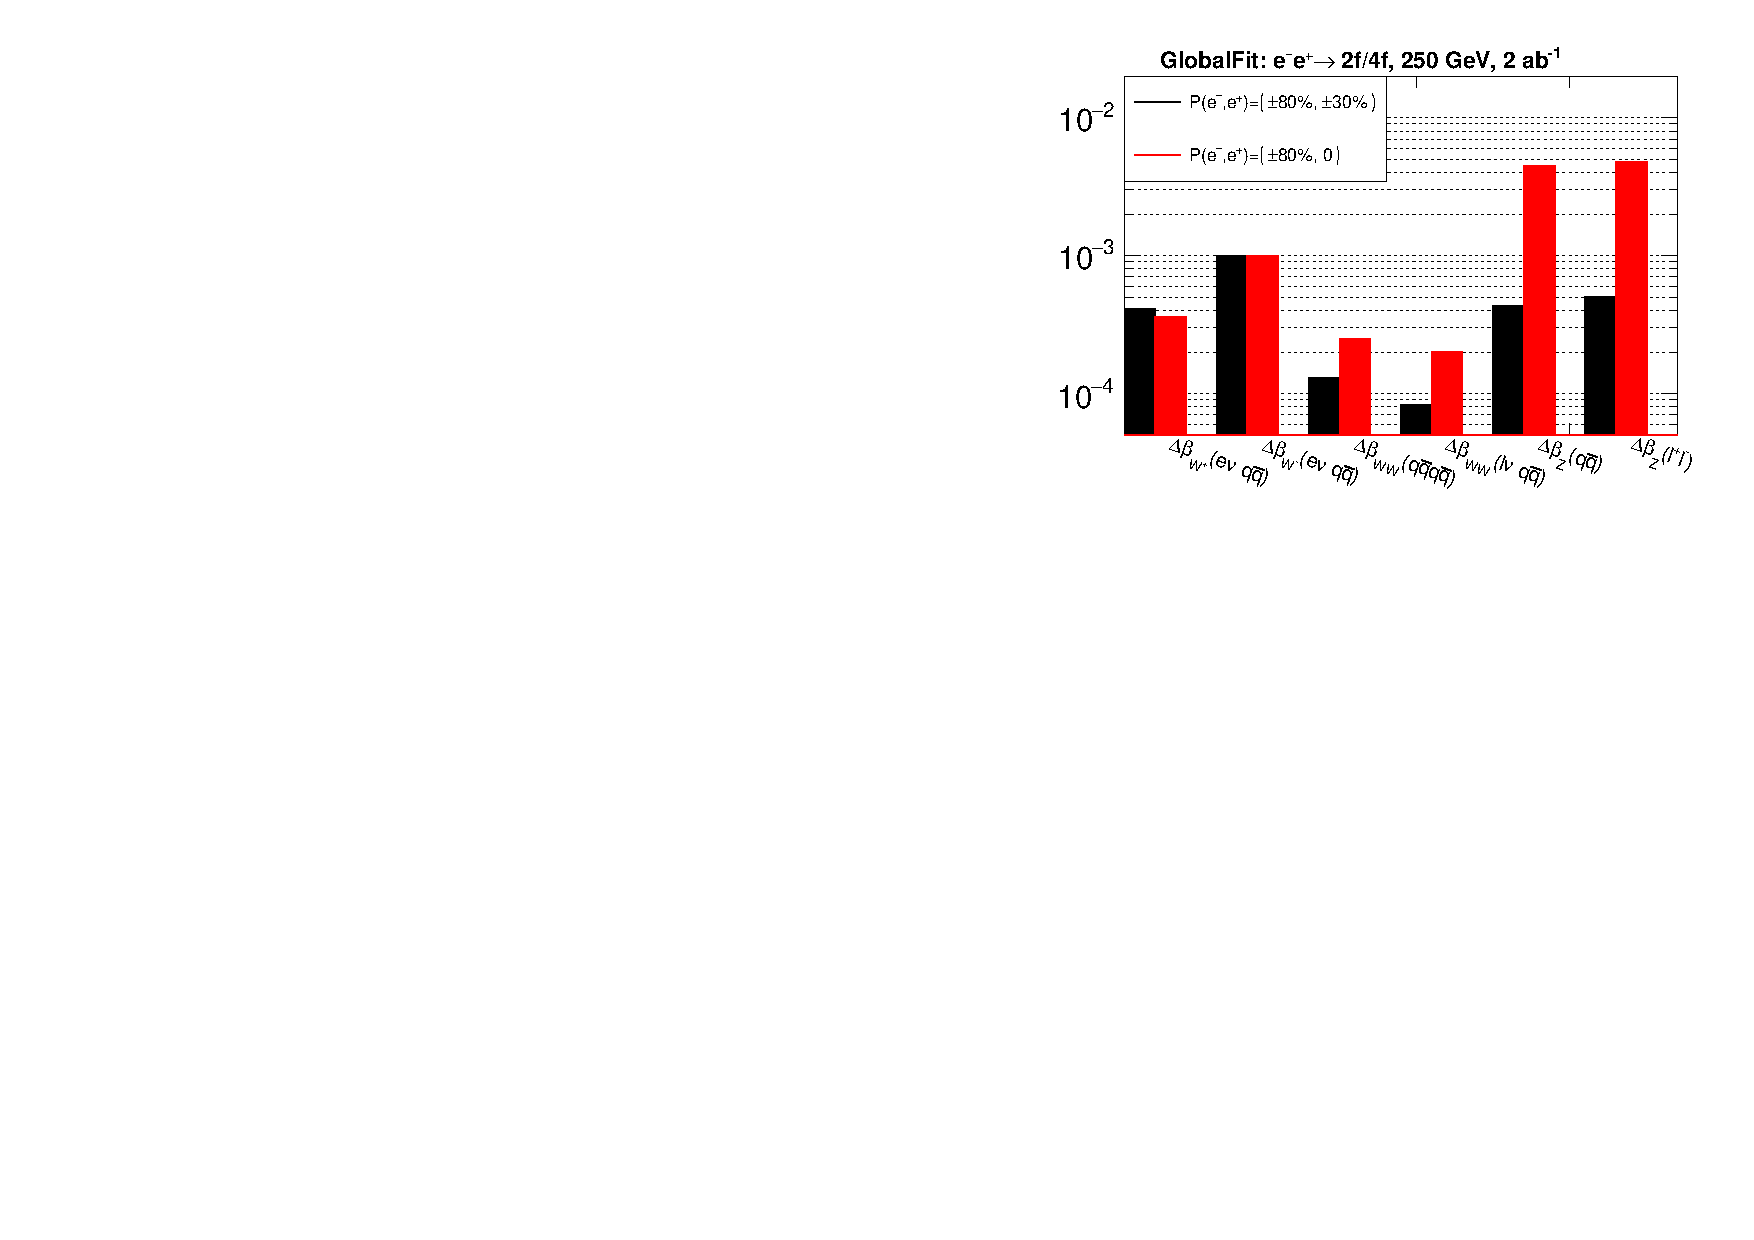
\includegraphics[width=0.95\linewidth]{./chapters/figures/beta_precision_upolarized.pdf}
		
\caption{Uncertainties $\Delta \beta$ on \ALR\ of various 2-fermion and 4-fermion processes as obtained from the global fit introduced in the text~\cite{bib:PhDRobert} with both beams polarised (with the standard 45\%/45\%/5\%/5\% sharing between the four helicity configurations) and in the absence of positron polarisation (with a 50\%/50\% sharing between the two remaining helicity configurations). In the absence of positron polarisation, the  uncertainties on \ALR\ increase by a factor 2 for $WW$ and by about a factor of 10 for 2-fermion processes. Alone the single-$W$ processes remain unaffected.}
\label{fig:beta_error_noposipol}
\end{figure}

\item{\textbf{Undetected biases:}} When considering the level of precision the ILC is aiming for, and even more so when attempting to go even further, even subtle biases can propagate to the results when not treated properly. As example, let's consider the case of operation with an unpolarised positron. In this case, one could assume that it would be fully sufficient to fix the nuisance parameters for the positron polarisation to zero. However it has been shown in~\cite{bib:PhDRobert} that in this case even a residual positron polarisation at the permille-level would already create a noticible bias on cross sections and asymmetries of the same order  of magnitude. This would make it hard to decide whether any possibly observed discrepancy from the SM expectation is a hint for new physics or due to a systematic effect. Therefore for ultimate precision, both beam polarisations should be treated as nuisance parameters independently of their absolute size.

\item {\textbf{Shape uncertainties and beam polarization:}} Uncertainties on the shape of distributions have been included in the WIMP search in the mono-photon channel~\cite{Habermehl:417605}. Figure~\ref{fig:polWIMPsys} shows the expected exclusion limit on the new physics scale $\Lambda$ as function of the WIMP mass for the same study cases as Fig.~\ref{fig:polWIMPstat}. The study includes a careful evaluation of the systematic uncertainties, comprising those on selection efficiencies, luminosity, beam energy (spectrum) and polarization as well as on the theoretical modelling of the background. 
The limit calculation uses a fractional event counting based on the observed energy spectrum of the selected photon candidates and considers normalisation and shape-dependent uncertainties as well as their (partial) correpations. The signal strength thereby has to be constrained on top of a significant irreducible background from $e^+e^- \to \nu\bar{\nu}\gamma$ and radiative low-angle Bhabha scattering. For increasing WIMP masses, the maximum possible energy of the ISR photons becomes lower. For the highest WIMP masses, the signal-free part of the spectrum becomes sufficiently large to constrain the nuisance parameters and thus to limited the impact of the systematic uncertainties. This effect is visible in form of the ``bump'' in the limit curves near $M_X=220$\,GeV. In case of the unpolarised data set, the effect starts to become visible already from $M_X=150$\,GeV onwards,
but the exclusion remains much weaker than in the polarised case. Comparison with Fig.~\ref{fig:polWIMPstat} shows that the benefit of polarisation in presence of systematic uncertainties goes significantly beyond the purely statistical $S/B$ effect. In particular it should be noted that when the systematic effects are included, the splitting of the total luminosity into four different data sets allows to set more stringent limits as if all luminosity would just be dedicated to the ``statistically-prefered'' helicity combination. In fact the result for only one helicity combination suffers as much from the systematic uncertainties as the unpolarised case, while in case of the polarisation mix, when four data sets with different helicities are used, the sensitivity is only affected veru weakly by the systematic uncertainties.



\begin{figure}
\centering
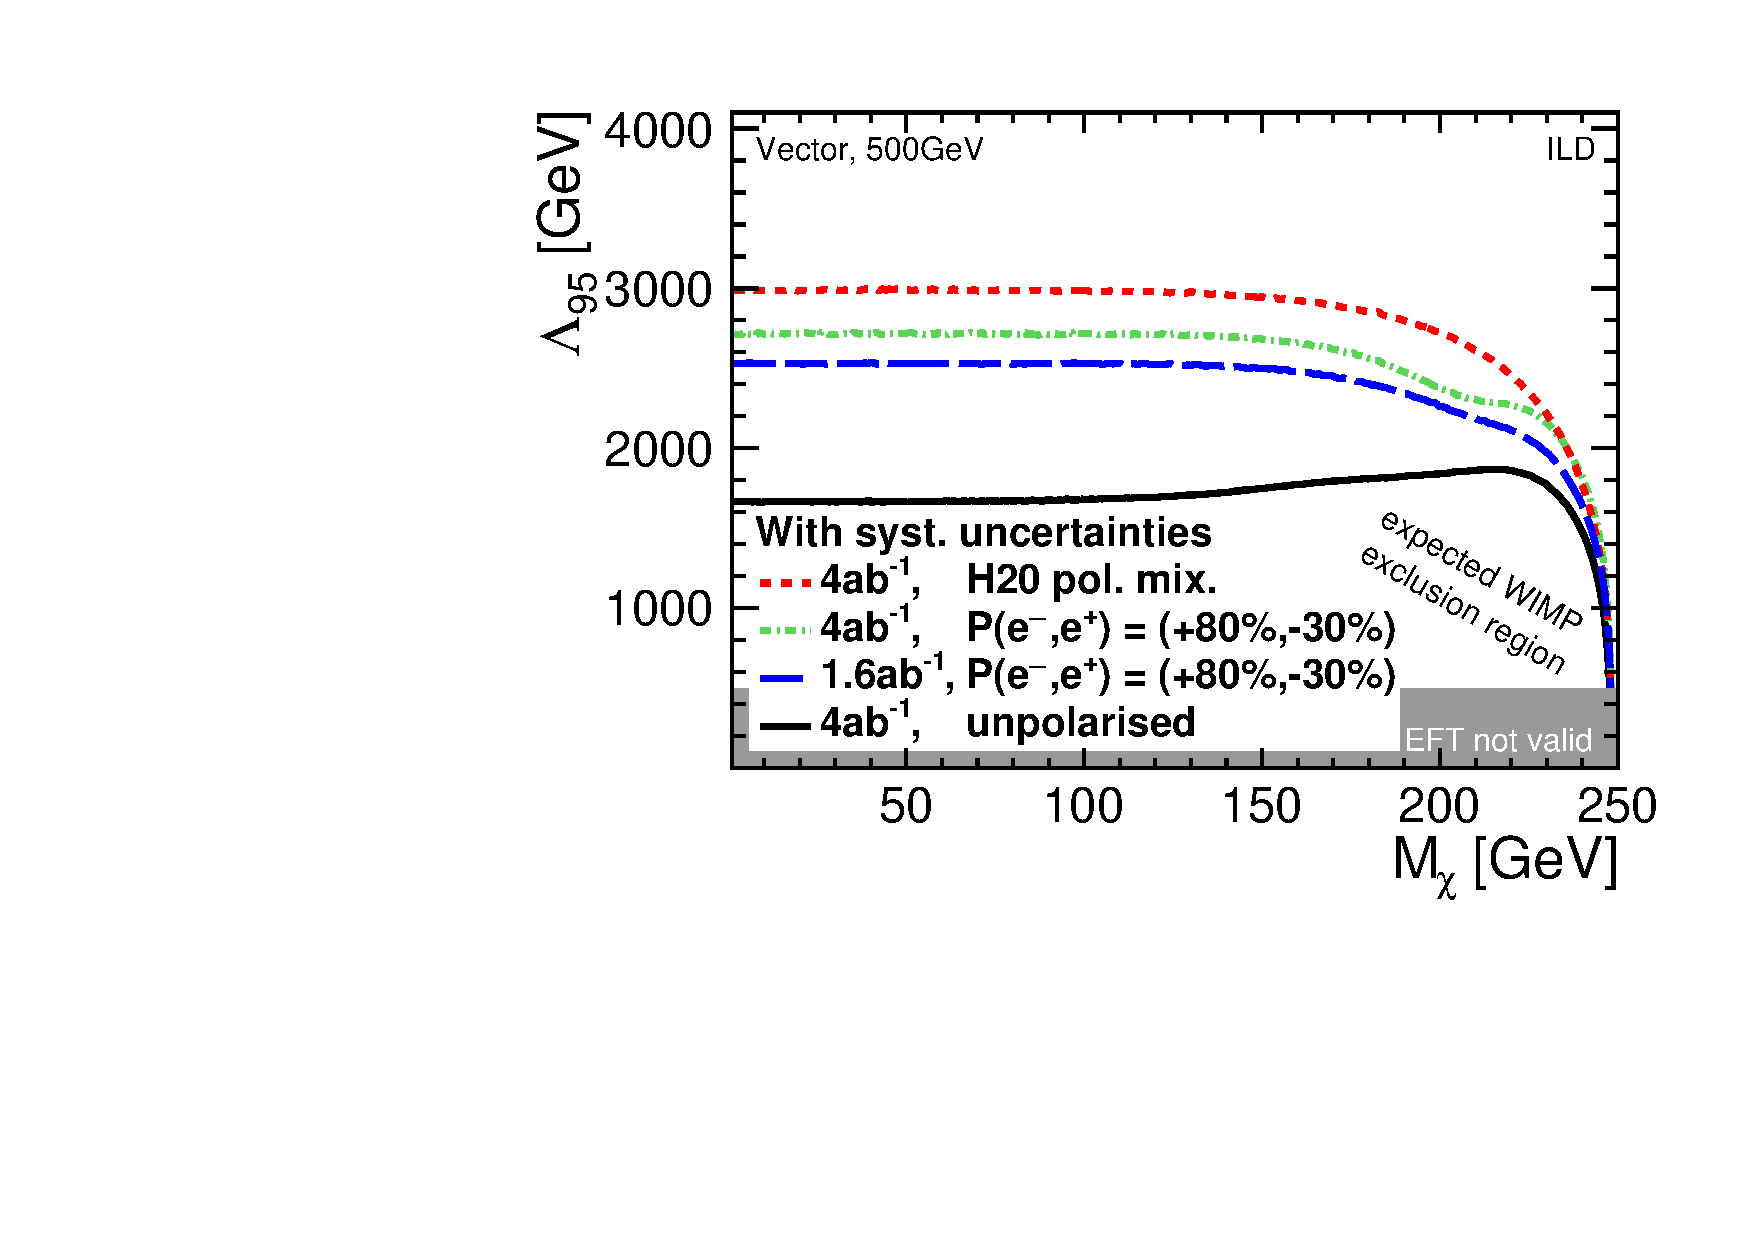
\includegraphics[width=0.95\linewidth]{./chapters/figures/vector_withSystematics.pdf}
		
\caption{Comparison of the reach of the search for WIMP production in the mono-photon channel for different assumptions on luminosity and polarization, {\em including} systematic uncertainties (see Sec.~\ref{sec:searches} for a description of the analysis)~\cite{Habermehl:417605}. }
\label{fig:polWIMPsys}
\end{figure}

\end{itemize}

\subsubsection{Systematic uncertainties considered in the Higgs coupling fit}
The Higgs coupling fits discussed in the following sections include the following systematic uncertainties:
\begin{itemize}
\item The luminosity at the ILC will be measured from low-angle Bhabha scattering with the help of a dedicated forward calorimeters, the LumiCals (see Sec.~\ref{sec:detectors} and Ref.~\cite{Abramowicz:2010bg}). This measurement is extremely sensitive to the exact alignment of the LumiCals on the two sides of the detector, as well as to beam backgrounds and has been studied in detailed simulations both for the ILC and for CLIC~\cite{Bozovic-Jelisavcic:2014aza, Lukic:2013fw}. Based on these studies, the resulting systematic uncertainty on all Higgs cross section and cross-section-times-braching-ratio measurements is assumed to be 0.1\%
\item Another 0.1\% is assumed for the net systematic effect of the finite knowledge of luminosity-weighted long-term average values of the beam polarisations at the $e^+e^-$ interaction point. While the Compton polarimeters in the Beam Delivery System resolve time-dependencies at the level of 0.25\%~\cite{Vormwald:2015hla, List:2015lsa}, also the effects of spin transport, misalignment of beam line magnets as well as depolarisation during the beam-beam interaction have been studied~\cite{Beckmann:2014mka}. The absolute scale of the luminosity-weighted average polarisation at the IP is finally calibrated from collision data, e.g.\ a global fit SM processes with a strong polarisation dependence~\cite{bib:PhDRobert}. 
\item Theoretical uncertainties are also assumed to have reched at the level of 0.1\% by the time of ILC operation {\color{red}[Any good \textbf{theoretical} arguments to add here?]}. This number is justified in case of polarised beams by the global fit study discussed above~\cite{bib:PhDRobert}, which showed that the absolute normalisations of cross sections and left-right asymetries can be controled  at this level. In the case of unpolarised beams, the theoretical uncertainties would require a much more detailed consideration.
\item As mentioned already at the beginning of Sec.~\ref{subsubsec:pol:systematics} experimental systematics on selection efficiencies, flavour tagging, detector calibrations etc of 1\% have already been reached at LEP in many cases. With the advances in detector technology and the larger integrated luminosity, we assume that for each data set at the ILC this can be reduced by a factor of 3 to 0.3\%. These 0.3\% are considered as net effect of all experimental uncertainties in the absence of beam polarisation.

In the presence of both beam polarisations, the net effect of systematic uncertainties has been shown to be smaller by factors between 2 and 10 due to the correlations between data sets with different beam polarisations as discussed in Sec.~\ref{subsubsec:pol:systematics}. Since the Higgs coupling fit does not yet comprise such a detailed treatment of systematic uncertainties and their correlations as the above mentioned global fit to 2-fermion and 4-fermion processes, we assume that, in presence of polarised beams, the net effect of the experimental uncertainties reduces to 0.1\%.
\end{itemize}


%%%%%%%% to be moved to IX C %%%%%%%%%%%%%%%%%%%%%%%%%%%%%

{\color{red}[THE FOLLOWING IS TO BE MOVED TO SECTION~\ref{subsec:lincirc}]}\\
Figure~\ref{fig:polWIMPmanhattans} shows the 95\% CL reach in new physics scale $\Lambda$ for pair production of a light ($M_{X} = 1$\,GeV) WIMP mediated by a vector operator for different assumptions on luminosity, energy and polarization 
as they are typical for linear and circular colliders. In particular the polarised
configurations al refer to the ILC reference running scenario H20, see Sec.~\ref{sec:runscenarios}. Input to the limit calculation is the ILC study performed in full detector simulation of the ILD detector concept described in~Sec.~\ref{sec:searches}, and its extrapolation to other center-of-mass energies~\cite{Habermehl:417605}. The study includes a careful evaluation of the systematic uncertainties, comprising those on selection efficiencies, luminosity, beam energy (spectrum) and polarization as well as on the theoretical modelling of the background. The limit calculation uses a fractional event counting based on the 
energy spectrum of the photon. It can be seen that at 250\,GeV, 2\,\iab\ with polarized beams offer a greater reach than 5 or even 10\,\iab\ without beam polarization. Even at a higher center-of-mass energy of 350\,GeV, about 10\,\iab\ of unpolarised data  would be required to catch up with 2\,\iab\ of polarised data at 250\,GeV. The higher center-of-mass energies reachable by linear colliders, in conjuction with beam polarisation, improve the reach considerably. For instance the reach of the full H20 running scenario of the ILC roughly doubles the reach in $\Lambda$ compared to the 250\,GeV stage.

\begin{figure}
\centering
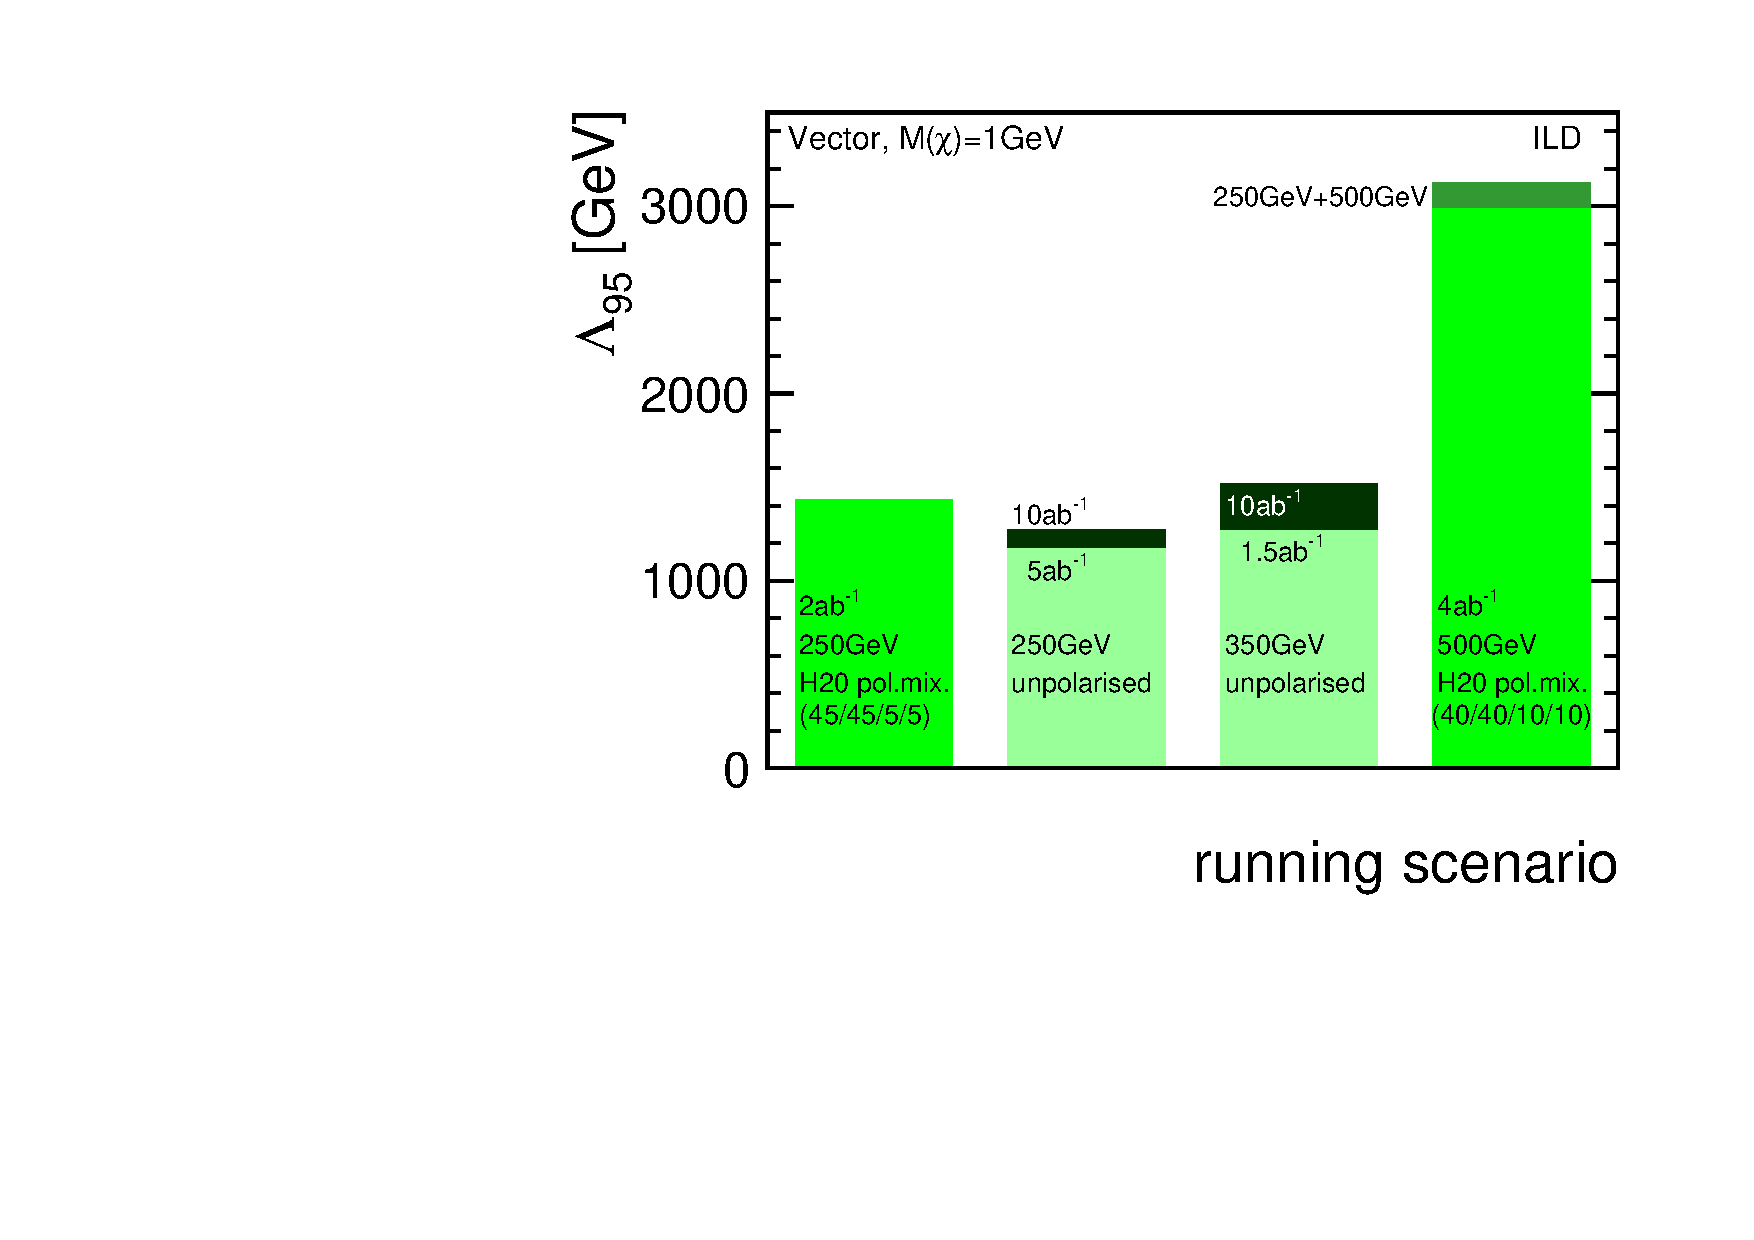
\includegraphics[width=0.95\linewidth]{./chapters/figures/manhattan_vector_v3.pdf}
		
\caption{{\color{red}[Michael, I think this plot and its description would better fit into section~\ref{subsec:lincirc}, but I didn't want to mess with `your' tex file. Please move it to your section if you like!]} Comparison of the reach for WIMP searches in the mono-photon channel for different assumptions on luminosity, polarization and energy, including systematic uncertainties (see Sec.~\ref{sec:searches} for a description of the analysis)~\cite{Habermehl:417605}. }
\label{fig:polWIMPmanhattans}
\end{figure}






Beam polarization is considered as an essential ingredient of the ILC physics program because of three important advantages:
\begin{enumerate}
\item Suppression of backgrounds and enhancement of signals
\item Analysis of the chiral properties
\item Control of systematic uncertainties
\end{enumerate}
The first two items often (but not always!) apply to a large extent already when only electron polarisation is available. 
However for the third aspect, the positron polarisation is crucial in many cases --- in particular whenever the left-right asymmetry \ALR\ itself is the physics observable, like \eg\ for 2-fermion processes (see Sec.~\ref{subsec:ew_ffana}) or for the Higgs precision measurements (see Sec.~\ref{subsec:ew_WWana}).
All three aspects will be discussed and illustrated with concrete physics examples in the following subsections. 

A comprehensive review of the role of polarization with many more examples can be found in~\cite{MoortgatPick:2005cw}, and a recent discussion of positron polarization in particular in~\cite{Fujii:2018mli}. 

%%%%%%%%%%%%%%%%%%%%%%%%%%%%%%%%%%%%%%%%%%%%%%%%%%%%%%%%%%%%%%%%%%%%%%%%%%%%5

\subsubsection{Suppression of backgrounds and enhancement of signals} 
\label{subsubsec:pol:s_over_b}
Due to the chiral structure of the weak interaction, and especially since right-handed fermions form isospin-singlets and therefore don't participate in charged current interactions, every $e^+e^-$ cross section depends on the chirality of the incoming beam particles.  For any given polarization of the electron and positron beams, \Pem\ and \Pep, respectively, the polarised cross section is caluculated from the chiral cross sections in the following way:
\begin{eqnarray}
\sigma_{\Pem\Pep} &=& \frac{1}{4}\bigl\{
     (1+\Pem)(1+\Pep) \quad \sigmaRR  \nonumber \\
&& + (1-\Pem)(1-\Pep) \sigmaLL \nonumber \\
&& + (1+\Pem)(1-\Pep) \sigmaRL \nonumber \\ 
&& + (1-\Pem)(1+\Pep) \sigmaLR \bigr\},
\label{eq:pol:xsec}
\end{eqnarray}


For charged current $t$-channel processes, like $e^+e^- \to W^+W^-$, $e^+e^- \to \nu_e\bar{\nu}_e$ or Higgs production via $WW$ fusion, only the \sigmaLR\ contribution is allowed, so that their rate can be dialed up or down by a factor 17 for $\Pmp=(\pm 80\%,\mp 30\%)$ (36 for $\Pmp=(\pm 80\%,\mp 60\%)$) via the choice of the polarisation sign. 

For $s$-channel processes in the SM, including Higgsstrahlung, \sigmaLR\ and \sigmaRL\ contribute. In this case, Eqn~\ref{eq:pol:xsec} can be reduced to
\begin{equation}
 \sigma_{\Pem\Pep} = 2 \sigma_0 (\Leff/\mathcal{L}) \left[1 - \ALR \Peff \right]
\label{eq:pol:xsecschan}
\end{equation}
Here, $\sigma_0$ is the unpolarized cross section and \ALR\ 
the left-right asymmetry, defined in Eqn.~\ref{eq:defALR}. \Leff\ and \Peff\  
are the effective luminosity and polarization, respectively, defined as
\begin{equation}
\Peff= \frac{\Pem - \Pep}{1 - \Pep\Pem}
\label{eq:def-leff-peff}
\quad\mbox{\rm and }\quad
\Leff=\frac{1}{2}(1 -\Pep\Pem)\L
\end{equation}

In practice, for $\Pmp=(\pm 80\%,\mp 30\%)$, $\Peff = \pm 89\%$ and $\Leff = 62\% \mathcal{L}$, whereas for $\Pmp=(0,0)$ and , $\Peff = 0$ and $\Leff = 50\% \mathcal{L}$, since in half of the cases a left-handed electron will meet a left-handed positron --- for which the cross section for $s$-channel processes is zero. 

With \ALR = 0.151 for Higgsstrahlung, this means that the cross section for $\Pmp=(-80\%,+30\%)$ is 41\% larger than the unpolarised cross section, while it is
still 7\% larger than the unpolarised cross section for the opposite sign combination  $\Pmp=(+80\%,-30\%)$. Since, as we saw above, important background processes like $e^+e^- \to W^+W^-$ are strongly suppressed in this configuration, the $\Pmp=(+80\%,-30\%)$ gives comparable and in some cases even better results than the $\Pmp=(-80\%,+30\%)$ configuration. 

However the signal-to-background ratio ($S/B$ or $S/sqrt{B}$) cannot be maximized for all processes at the same time. But it is very important to realize that the combination of a high-$S/B$ data set with a low-$S/B$ data set is statistically {\em not} equivalent to taking 
the same amount of data with the average $S/B$, simply because significances don't add up linearly. Therefore the overall precision increases even if the total intergrated luminosity is split between ``optimal'' and ``non-optimal'' configurations. 

This is illustrated in Fig.~\ref{fig:polWIMPstat}, which compares the reach of the search for WIMP production in the mono-photon channel for different assumptions on luminosity and polarization (see Sec.~\ref{sec:searches} for a description of the analysis). It clearly shows the large increase in sensitivity for \Pmp=(+80\%, -30\%) w.r.t.\ the unpolarised case, and that the result for splitting the data on all four helicity configurations as forseen in the H20 running scenario, albeit completely dominated by the 1.6\,\iab\ collected with \Pmp=(+80\%, -30\%), is still probing significantly higher scales than the unpolarised case. Note that this figure omits all systematic uncertainties in order to highlight the statistical $S/B$ effect. 
\begin{figure}
\centering
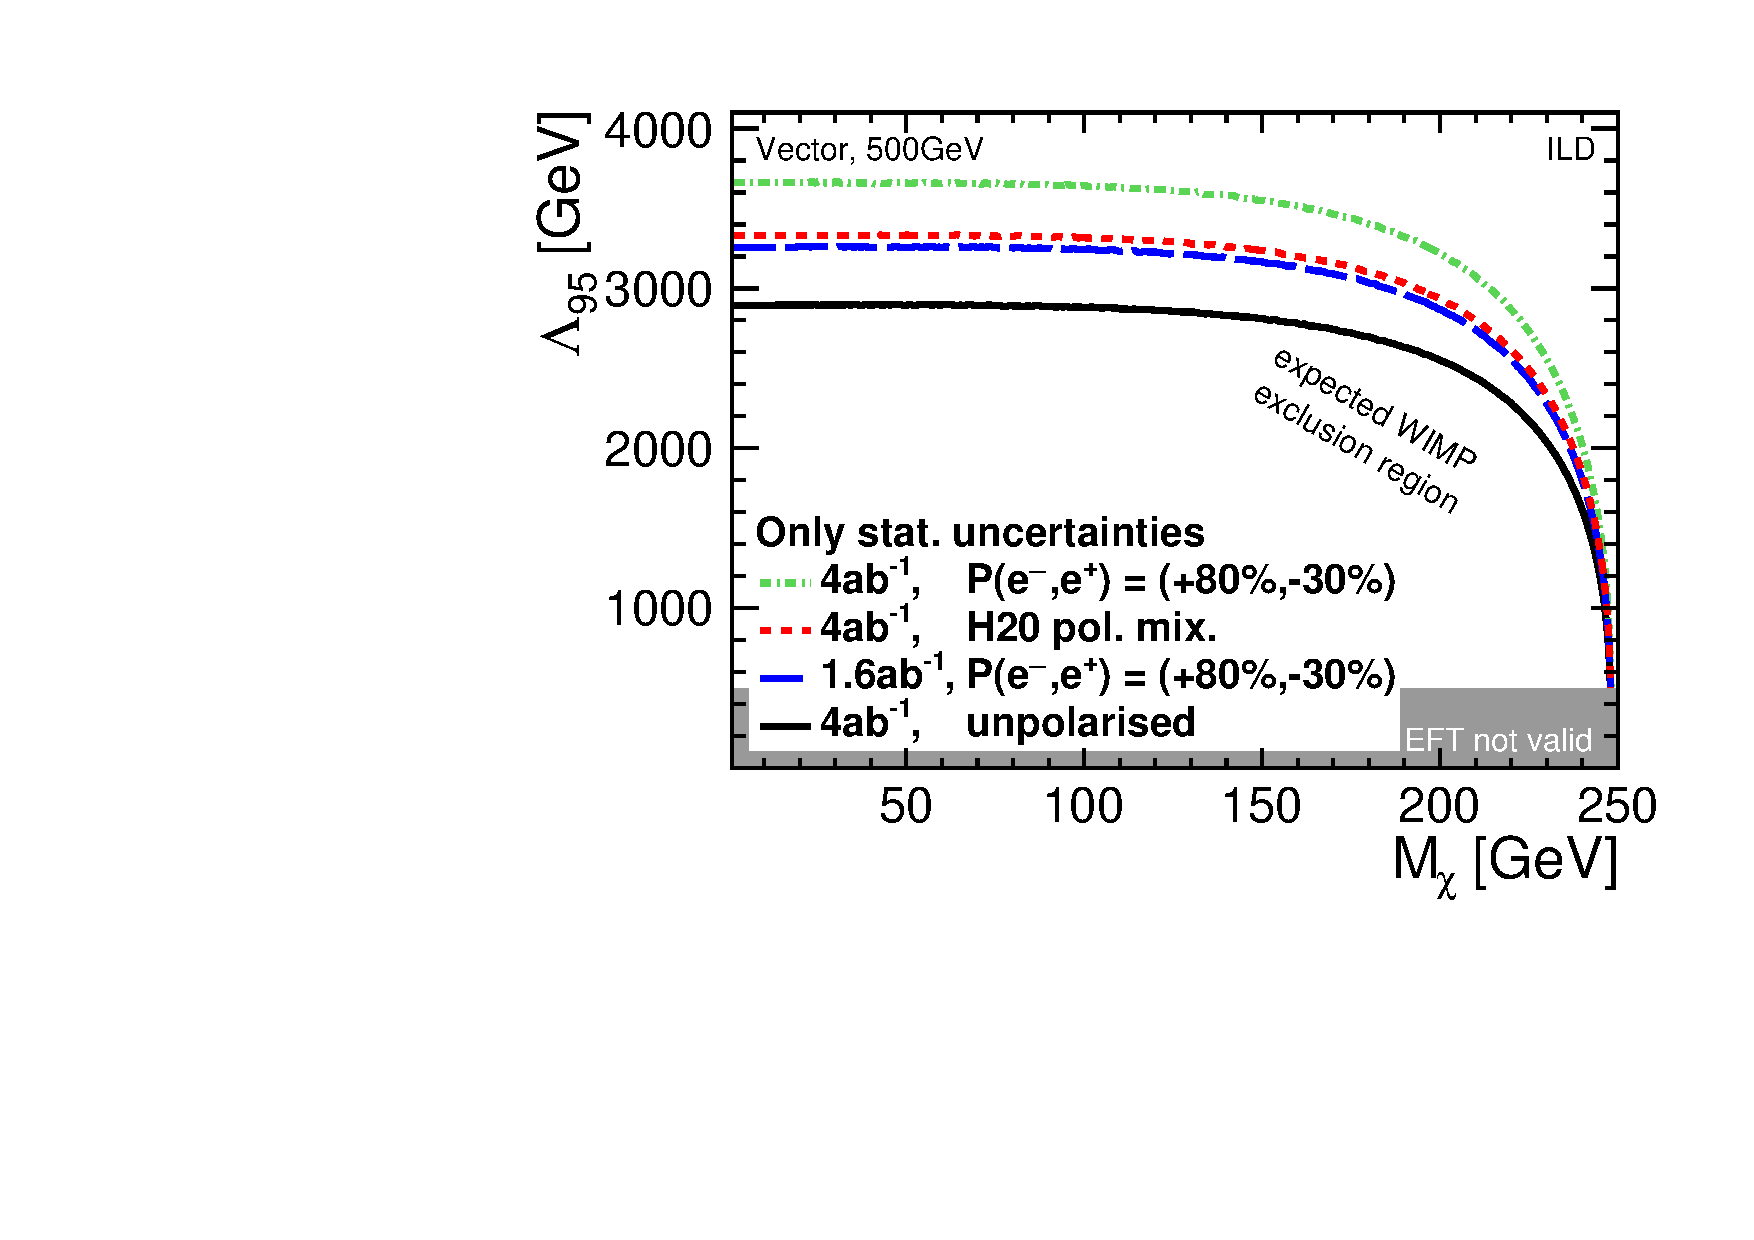
\includegraphics[width=0.95\linewidth]{./chapters/figures/vector_noSystematics.pdf}
		
\caption{Comparison of the reach of the search for WIMP production in the mono-photon channel for different assumptions on luminosity and polarization (see Sec.~\ref{sec:searches} for a description of the analysis)~\cite{Habermehl:417605}. Note that this plot is considering {\em statistical uncertainties only}. The corresponding comparison {\em including systematic uncertainties} is shown in Fig.~\ref{fig:polWIMPsys}.}
\label{fig:polWIMPstat}
\end{figure}

%%%%%%%%%%%%%%%%%%%%%%%%%%%%%%%%%%%%%%%%%%%%%%%%%%%%%%%%%%%%%%%%%%%%%%%%%%%%5

\subsubsection{Analysis of chiral properties} 
\label{subsubsec:pol:chiral}
Beam polarisation is essential to analyze the chiral structure of SM processes in search for deviations from a pure $V-A$ structure due to new physics contributions --- and, in case of a discovery of new particles at the LHC or the ILC itself, of these new particles and their interaction. The list of example applications is long and comprises for instance:
\begin{itemize}
\item Measurements fermion couplings in 2-fermion production: Beam polarisation is essential to disentangle the left- and right-handed couplings of each fermion species to the photon and the $Z$ boson, as discussed in Sec.~\ref{subsec:ew_ffana}. 
\item Measurements of triple gauge couplings: With both beams polarized and using various orientations of the polarisation vectors, all 14 complex couplings (thus 28 real parameters) of the most general Lagrangian for triple gauge vertices, including $CP$ violation, can be extracted simultaneously, as  discussed in Sec.~\ref{subsec:ew_WWana}.
\item Higgs coupling determination: The left-right asymmetry of the $ZH$ cross section has been found to be an important ingredient for constraining the full set of $CP$ conserving dimension-6 operators consistent with $SU(2) \times\ U(1)$ symmetry. This will be discussed in detail in Sec.~\ref{sec:global}.
\item Generic BSM effects: The chiral structure of physics beyond the SM is apriory not known - it could be similar to the SM or completely different. When parametrising new physics in terms of effective operators, the tensor structure of the operator immediately relates to the chiral cross sections: For instance the $s$-channel exchange of a vector mediator allows only for \sigmaLR\ and \sigmaRL\ by angular momentum conservation,
while the exchange of a scalar also has non-zero \sigmaLL\ and \sigmaRR. Since these
vanish in the SM, like-sign polarisation configurations are extremely sensitive to 
such types of new interactions. An example is e.g.\ the distinction between different WIMP models in the mono-photon channel, as discussed in Sec.~\ref{subsec:searches_monophoton}.
\end{itemize}  
% Many more applications can be found e.g.\ in~\cite{MoortgatPick:2005cw, Fujii:2018mli}. 

%%%%%%%%%%%%%%%%%%%%%%%%%%%%%%%%%%%%%%%%%%%%%%%%%%%%%%%%%%%%%%%%%%%%%%%%%%%%5

\subsubsection{Control of systematic uncertainties} 
\label{subsubsec:pol:systematics}

Last but not least, the redundancies provided by the combination of data sets with different beam polarization configurations are invaluable for the control of systematics uncertainties. Thereby it important to always have one more degree of freedom that (statistically) absolutely required: For physics measurements which do not aim at the analysis of a chiral structure, e.g.\ measurements of total unpolarised cross sections, two data sets with with different polarisations (e.g.\ $\Pmp=(\pm 80\%, \mp 30\%)$ or $\Pmp=(\pm 80\%, 0)$ often suffice to constrain the most important nuisance parameters. However if the chiral structure itself is among the observables, e.g.\ when measuring \ALR\ of 2-fermion processes or of Higgsstrahlung, one flip of the polarisation sign(s) is already contained in the observable itself, and thus a non-zero positron polarisation becomes essential to provide enough independent information to constrain nuisance parameters.

The evaluation of systematic uncertainties for experiments which have not yet been built is a difficult task and will to some extent always remain guess-work until real data have been taken. Important is therefore to include the experience from previous $e^+e^-$ experiments, especially at LEP, where many uncertainties could be controled to a typical level of 1\%. Assuming that the same level can be reached at future $e^+e^-$ colliders, detailed studies of systematic uncertainties at the ILC have concentrated on cases where the statistical uncertainties are expected to be significantly below 1\%, and on searches in channels with large irreducible backgrounds. An example for the first case is a global analysis of total rates and differential distributions of various 2-fermion and 4-fermion SM processes, extracting simultaneously the total unpolarised cross sections, the relevant left-right asymmetries, the beam polariations and the charged triple gauge couplings, see Sec.~\ref{subsec:ew_WWana} and Ref.~\cite{bib:PhDRobert}. An example for the second category is the WIMP search in the mono-photon channel, see Sec.~\ref{sec:searches} and Ref.~\cite{Habermehl:417605}. 

In the remainder of this section we will highlight the relative impact of the beam polarisation on the control of systematic uncertainties using these two studies as examples. The consequences for the treatment of systematic uncertainties in the Higgs coupling fit will be discussed in the next subsection.

\begin{itemize}
\item {\textbf{Fast-helicity reversal and correlations between data sets:}} The design of the ILC includes the capability to flip the sign of the two beam polarisations independently and on a train-by-train basis, as introduced in Sec.~\ref{par:beampol}. This helicity reversal is fast compared to typical time-scales of changes in the configuration, calibration and alignment of the detector and the accelerator, and thus data sets with the same beam energy but different beam helicities can be considered as being collected ``quasi-concurrently''. Therefore, many of the experimental systematic effects will be correlated to a large degree between data sets with different polarisations. Note that this does not apply for data sets with different center-of-mass energies, which are collected after each other, typically in different years, and thus systematic effects can in general not be expected to be correlated between such data sets.
Similarly, also most theoretical uncertainties will be correlated between same-energy-different-polarisation data sets, apart from those which directly concern the dependence of the polarised cross sections on the beam polarisations, so effectively any uncertainty to Eqn.~\ref{eq:pol:xsec} {\color{red} [JL: I can't think of any uncertainty to this very basic relation, but I don't dare to say that there is none - comments welcome!]}.  

As example, Fig.~\ref{fig:alpha_error_corr_uncorr} shows the uncertainties $\Delta \alpha $ on the unpolarised cross sections of various 2-fermion and 4-fermion processes as obtained from the global fit introduced above~\cite{bib:PhDRobert}, for the example of a 1\% uncertainty on selection efficiencies and purities, each. In the pesence of beam polarisation, it is assumed that only 10\%, thus 0.1\%, remain uncorrelated between the data sets of different polarisations. In absence of beam polarisation, there are no data sets with correlated systematic uncertainties, and the impact on the cross section uncertainties increases by a factor of 2 for $WW$ and single-$W$ processes, and a factor of 5 for $s$-channel $Z/\gamma$ exchange.
\begin{figure}
\centering
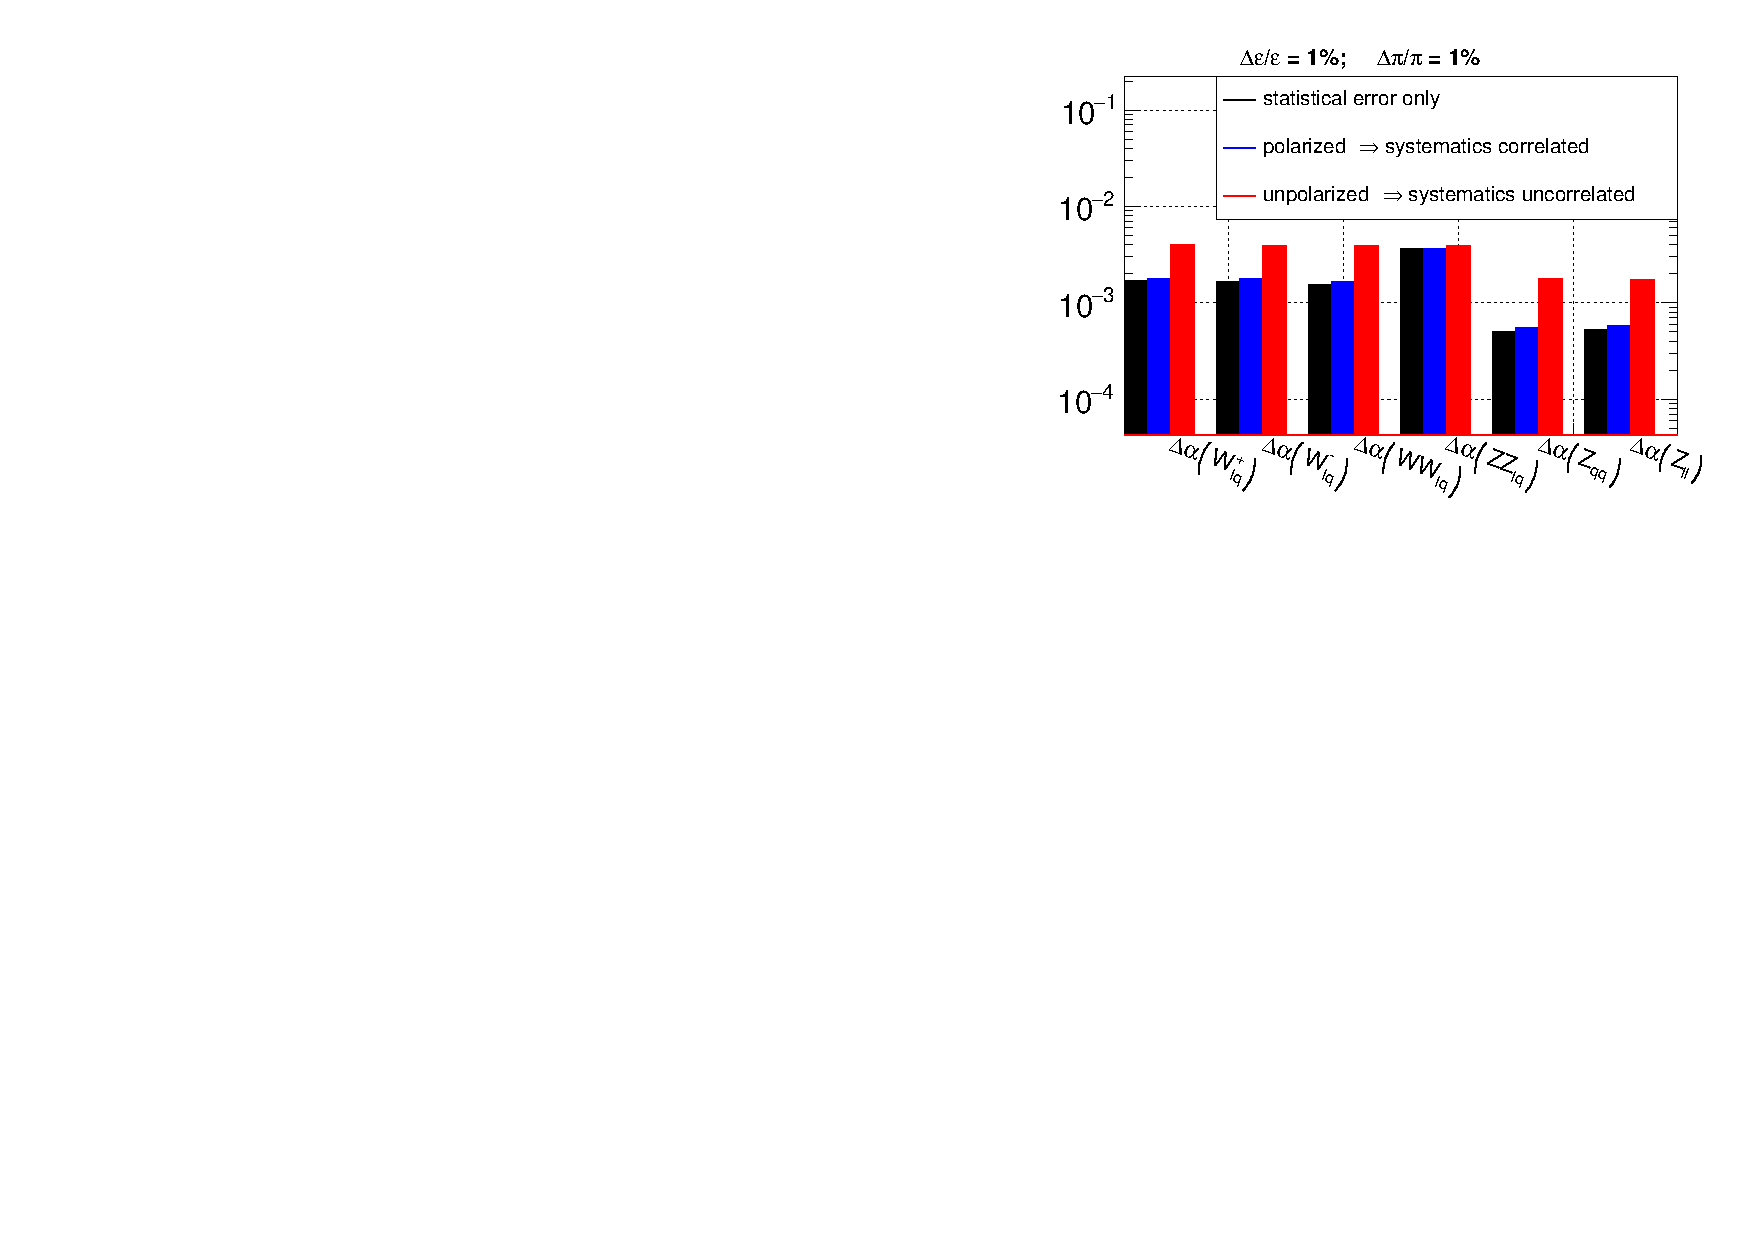
\includegraphics[width=0.95\linewidth]{./chapters/figures/ElectroWeakSysDependency_alpha_short.pdf}
		
\caption{Uncertainties on the unpolarised cross sections of various 2-fermion and 4-fermion processes as obtained from the global fit introduced in the text~\cite{bib:PhDRobert}, assuming a systematic uncertainty of 1\% on the selection efficiencies and purities, each. In the case of polarised beams, it is assumed that only 10\% of the uncertainty is uncorrelated between data sets - in this case the impact of the systematic uncertainties is minimal. Without the redundancies provided by data sets with correlated systematic uncertainties, the total uncertainties increase by a factor 2 for $WW$ and single-$W$ processes and a factor of 5 for 2-fermion processes.}
\label{fig:alpha_error_corr_uncorr}
\end{figure}

Note that this example so far only considers normalisation uncertainties. When adding shape uncertainties, however, the benefit from the redundacy offered by several data sets with correlated systematic effects is expected to be even more pronounced than in the current case of only normalisation uncertainties, since the shape uncertainties will reduce the information which can be extracted from the  differential distributions included in the fit.  

\item {\textbf{Impact of positron polarisation on \ALR\ measurement:}} The left-right asymmetries \ALR\ themselves are obviously only accessible when at least electron beam polarisation is available. Still the positron polarisation is crucial in order to reach ultimate precision on \ALR, as illustrated in Fig.~\ref{fig:beta_error_noposipol}, again from the global fit to 2- and 4-fermion processes. In this example, no detector or theory systematics are included, only the exact polarisation values are treated as nuisance parameters. It can be seen that in the absence of positron polarisation, the uncertainties on \ALR\ increase by 2 factor 2 on $WW$ production and by a factor of $10$ on $s$-channel $Z$ exchange. only the single-$W$ processes remain unaffected.


\begin{figure}
\centering
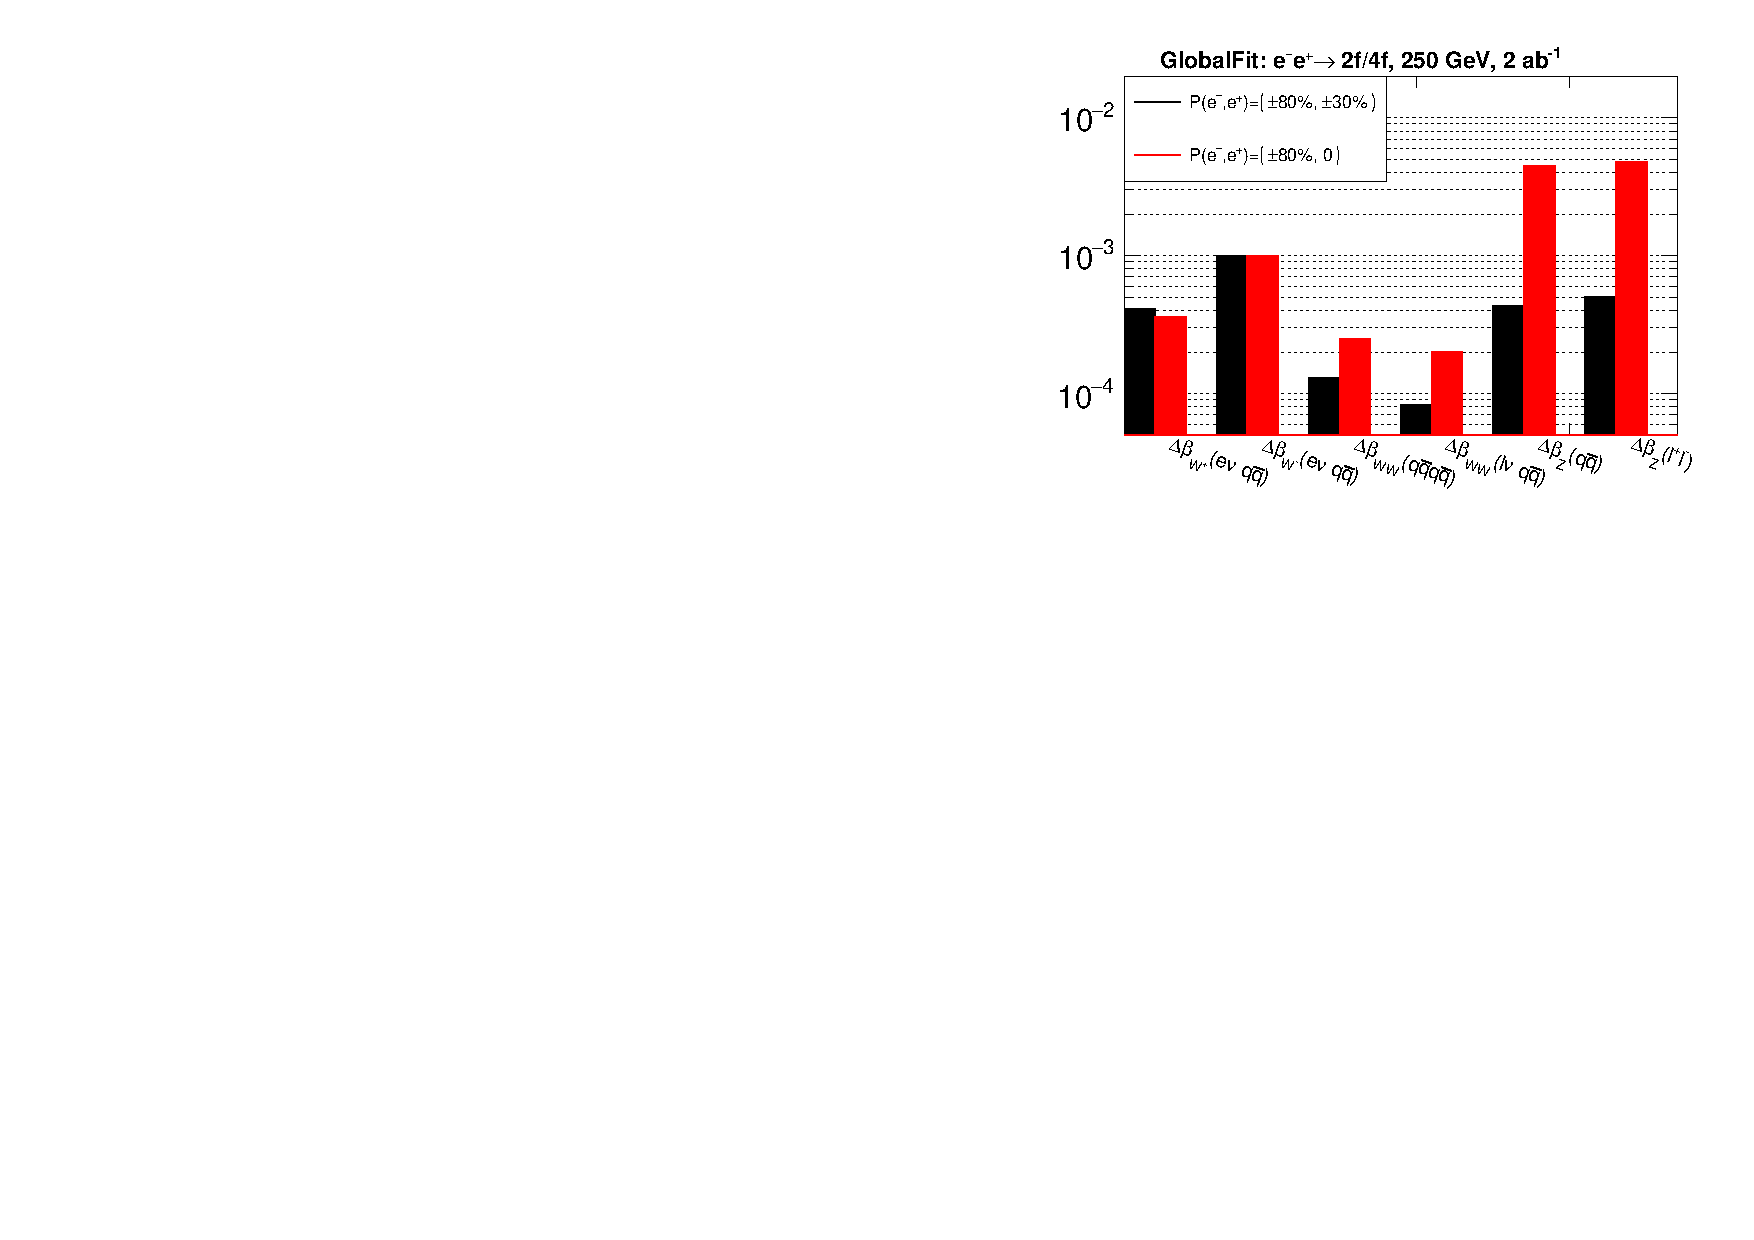
\includegraphics[width=0.95\linewidth]{./chapters/figures/beta_precision_upolarized.pdf}
		
\caption{Uncertainties $\Delta \beta$ on \ALR\ of various 2-fermion and 4-fermion processes as obtained from the global fit introduced in the text~\cite{bib:PhDRobert} with both beams polarised (with the standard 45\%/45\%/5\%/5\% sharing between the four helicity configurations) and in the absence of positron polarisation (with a 50\%/50\% sharing between the two remaining helicity configurations). In the absence of positron polarisation, the  uncertainties on \ALR\ increase by a factor 2 for $WW$ and by about a factor of 10 for 2-fermion processes. Alone the single-$W$ processes remain unaffected.}
\label{fig:beta_error_noposipol}
\end{figure}

\item{\textbf{Undetected biases:}} When considering the level of precision the ILC is aiming for, and even more so when attempting to go even further, even subtle biases can propagate to the results when not treated properly. As example, let's consider the case of operation with an unpolarised positron. In this case, one could assume that it would be fully sufficient to fix the nuisance parameters for the positron polarisation to zero. However it has been shown in~\cite{bib:PhDRobert} that in this case even a residual positron polarisation at the permille-level would already create a noticible bias on cross sections and asymmetries of the same order  of magnitude. This would make it hard to decide whether any possibly observed discrepancy from the SM expectation is a hint for new physics or due to a systematic effect. Therefore for ultimate precision, both beam polarisations should be treated as nuisance parameters independently of their absolute size.

\item {\textbf{Shape uncertainties and beam polarization:}} Uncertainties on the shape of distributions have been included in the WIMP search in the mono-photon channel~\cite{Habermehl:417605}. Figure~\ref{fig:polWIMPsys} shows the expected exclusion limit on the new physics scale $\Lambda$ as function of the WIMP mass for the same study cases as Fig.~\ref{fig:polWIMPstat}. The study includes a careful evaluation of the systematic uncertainties, comprising those on selection efficiencies, luminosity, beam energy (spectrum) and polarization as well as on the theoretical modelling of the background. 
The limit calculation uses a fractional event counting based on the observed energy spectrum of the selected photon candidates and considers normalisation and shape-dependent uncertainties as well as their (partial) correpations. The signal strength thereby has to be constrained on top of a significant irreducible background from $e^+e^- \to \nu\bar{\nu}\gamma$ and radiative low-angle Bhabha scattering. For increasing WIMP masses, the maximum possible energy of the ISR photons becomes lower. For the highest WIMP masses, the signal-free part of the spectrum becomes sufficiently large to constrain the nuisance parameters and thus to limited the impact of the systematic uncertainties. This effect is visible in form of the ``bump'' in the limit curves near $M_X=220$\,GeV. In case of the unpolarised data set, the effect starts to become visible already from $M_X=150$\,GeV onwards,
but the exclusion remains much weaker than in the polarised case. Comparison with Fig.~\ref{fig:polWIMPstat} shows that the benefit of polarisation in presence of systematic uncertainties goes significantly beyond the purely statistical $S/B$ effect. In particular it should be noted that when the systematic effects are included, the splitting of the total luminosity into four different data sets allows to set more stringent limits as if all luminosity would just be dedicated to the ``statistically-prefered'' helicity combination. In fact the result for only one helicity combination suffers as much from the systematic uncertainties as the unpolarised case, while in case of the polarisation mix, when four data sets with different helicities are used, the sensitivity is only affected veru weakly by the systematic uncertainties.



\begin{figure}
\centering
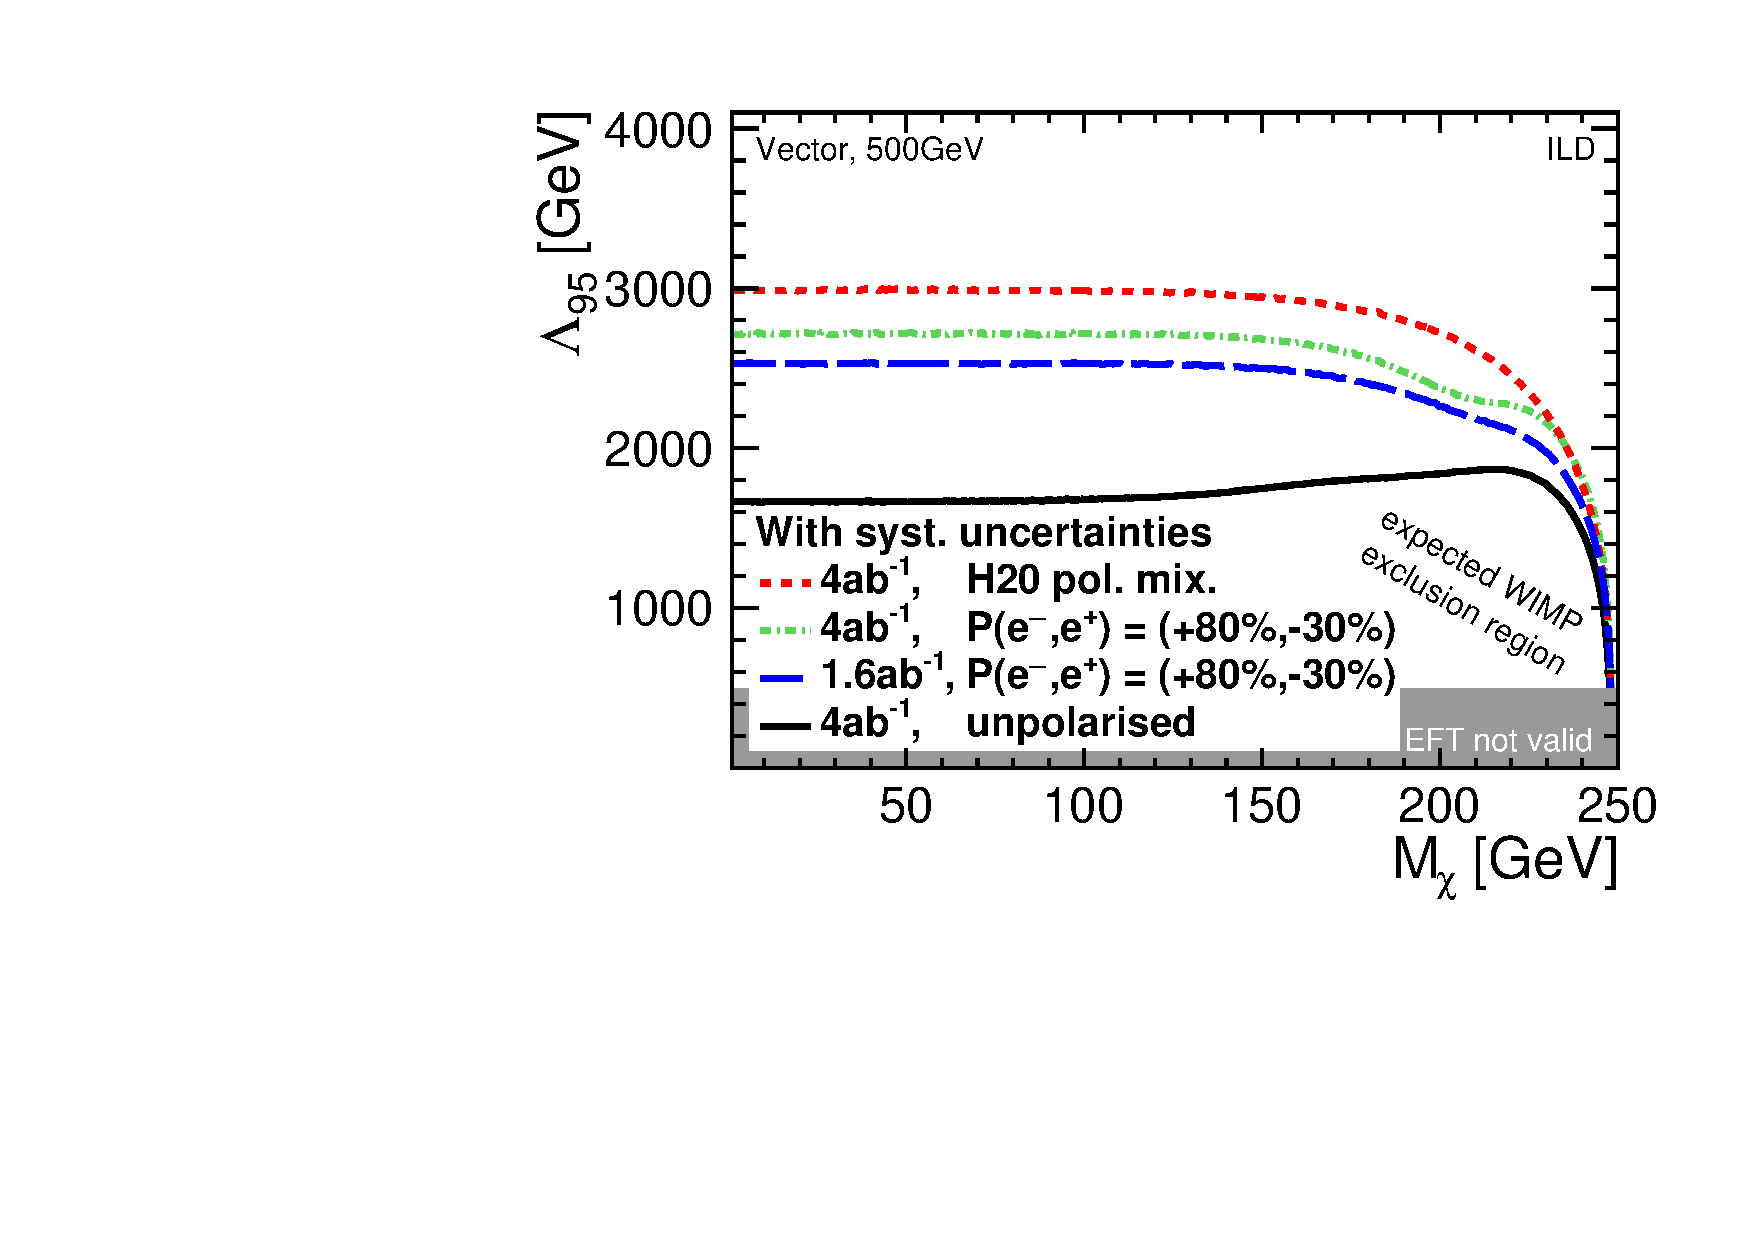
\includegraphics[width=0.95\linewidth]{./chapters/figures/vector_withSystematics.pdf}
		
\caption{Comparison of the reach of the search for WIMP production in the mono-photon channel for different assumptions on luminosity and polarization, {\em including} systematic uncertainties (see Sec.~\ref{sec:searches} for a description of the analysis)~\cite{Habermehl:417605}. }
\label{fig:polWIMPsys}
\end{figure}

\end{itemize}

\subsubsection{Systematic uncertainties considered in the Higgs coupling fit}
The Higgs coupling fits discussed in the following sections include the following systematic uncertainties:
\begin{itemize}
\item The luminosity at the ILC will be measured from low-angle Bhabha scattering with the help of a dedicated forward calorimeters, the LumiCals (see Sec.~\ref{sec:detectors} and Ref.~\cite{Abramowicz:2010bg}). This measurement is extremely sensitive to the exact alignment of the LumiCals on the two sides of the detector, as well as to beam backgrounds and has been studied in detailed simulations both for the ILC and for CLIC~\cite{Bozovic-Jelisavcic:2014aza, Lukic:2013fw}. Based on these studies, the resulting systematic uncertainty on all Higgs cross section and cross-section-times-braching-ratio measurements is assumed to be 0.1\%
\item Another 0.1\% is assumed for the net systematic effect of the finite knowledge of luminosity-weighted long-term average values of the beam polarisations at the $e^+e^-$ interaction point. While the Compton polarimeters in the Beam Delivery System resolve time-dependencies at the level of 0.25\%~\cite{Vormwald:2015hla, List:2015lsa}, also the effects of spin transport, misalignment of beam line magnets as well as depolarisation during the beam-beam interaction have been studied~\cite{Beckmann:2014mka}. The absolute scale of the luminosity-weighted average polarisation at the IP is finally calibrated from collision data, e.g.\ a global fit SM processes with a strong polarisation dependence~\cite{bib:PhDRobert}. 
\item Theoretical uncertainties are also assumed to have reched at the level of 0.1\% by the time of ILC operation {\color{red}[Any good \textbf{theoretical} arguments to add here?]}. This number is justified in case of polarised beams by the global fit study discussed above~\cite{bib:PhDRobert}, which showed that the absolute normalisations of cross sections and left-right asymetries can be controled  at this level. In the case of unpolarised beams, the theoretical uncertainties would require a much more detailed consideration.
\item As mentioned already at the beginning of Sec.~\ref{subsubsec:pol:systematics} experimental systematics on selection efficiencies, flavour tagging, detector calibrations etc of 1\% have already been reached at LEP in many cases. With the advances in detector technology and the larger integrated luminosity, we assume that for each data set at the ILC this can be reduced by a factor of 3 to 0.3\%. These 0.3\% are considered as net effect of all experimental uncertainties in the absence of beam polarisation.

In the presence of both beam polarisations, the net effect of systematic uncertainties has been shown to be smaller by factors between 2 and 10 due to the correlations between data sets with different beam polarisations as discussed in Sec.~\ref{subsubsec:pol:systematics}. Since the Higgs coupling fit does not yet comprise such a detailed treatment of systematic uncertainties and their correlations as the above mentioned global fit to 2-fermion and 4-fermion processes, we assume that, in presence of polarised beams, the net effect of the experimental uncertainties reduces to 0.1\%.
\end{itemize}


%%%%%%%% to be moved to IX C %%%%%%%%%%%%%%%%%%%%%%%%%%%%%

{\color{red}[THE FOLLOWING IS TO BE MOVED TO SECTION~\ref{subsec:lincirc}]}\\
Figure~\ref{fig:polWIMPmanhattans} shows the 95\% CL reach in new physics scale $\Lambda$ for pair production of a light ($M_{X} = 1$\,GeV) WIMP mediated by a vector operator for different assumptions on luminosity, energy and polarization 
as they are typical for linear and circular colliders. In particular the polarised
configurations al refer to the ILC reference running scenario H20, see Sec.~\ref{sec:runscenarios}. Input to the limit calculation is the ILC study performed in full detector simulation of the ILD detector concept described in~Sec.~\ref{sec:searches}, and its extrapolation to other center-of-mass energies~\cite{Habermehl:417605}. The study includes a careful evaluation of the systematic uncertainties, comprising those on selection efficiencies, luminosity, beam energy (spectrum) and polarization as well as on the theoretical modelling of the background. The limit calculation uses a fractional event counting based on the 
energy spectrum of the photon. It can be seen that at 250\,GeV, 2\,\iab\ with polarized beams offer a greater reach than 5 or even 10\,\iab\ without beam polarization. Even at a higher center-of-mass energy of 350\,GeV, about 10\,\iab\ of unpolarised data  would be required to catch up with 2\,\iab\ of polarised data at 250\,GeV. The higher center-of-mass energies reachable by linear colliders, in conjuction with beam polarisation, improve the reach considerably. For instance the reach of the full H20 running scenario of the ILC roughly doubles the reach in $\Lambda$ compared to the 250\,GeV stage.

\begin{figure}
\centering
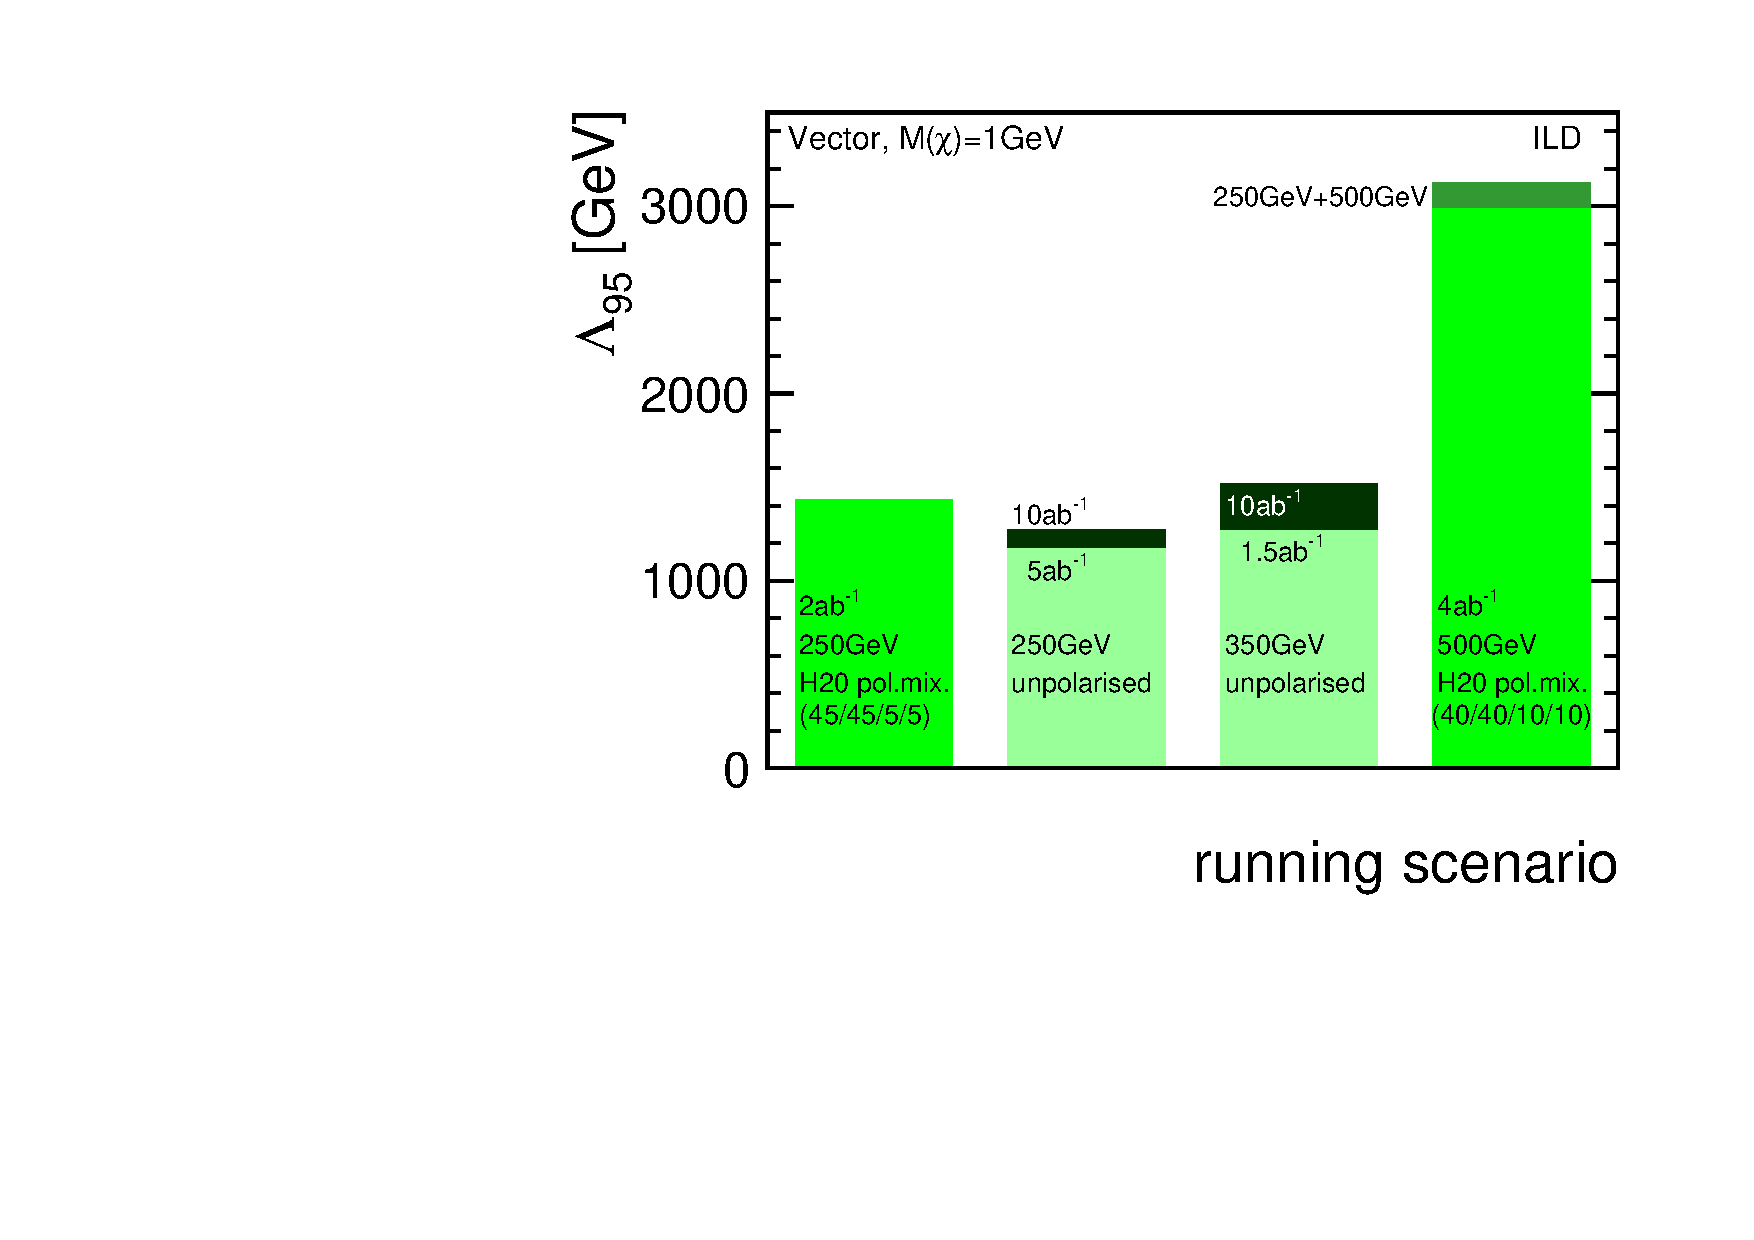
\includegraphics[width=0.95\linewidth]{./chapters/figures/manhattan_vector_v3.pdf}
		
\caption{{\color{red}[Michael, I think this plot and its description would better fit into section~\ref{subsec:lincirc}, but I didn't want to mess with `your' tex file. Please move it to your section if you like!]} Comparison of the reach for WIMP searches in the mono-photon channel for different assumptions on luminosity, polarization and energy, including systematic uncertainties (see Sec.~\ref{sec:searches} for a description of the analysis)~\cite{Habermehl:417605}. }
\label{fig:polWIMPmanhattans}
\end{figure}






\subsection{Comparison of run scenarios for linear and circular $\ee$ collliders}
\label{subsec:lincirc}





\subsection{Comparison of the ILC and the HL-LHC Higgs capabilities}
\label{subsec:higgs:ilclhc}











It is appropriate to compare the capabilities of the ILC for precision
Higgs measurement to those of the HL-LHC.  Since the ILC is planned as
an expensive new accelerator project, it should be justified on the
basis that it will qualitatively advance our knowledge of the Higgs
boson over what is possible from the LHC in its high luminosity stage.  
This section will present several such comparisons.

The goal of the ILC is not simply to achieve a high degree of
precision in the measurement of Higgs boson couplings; it is to
discover deviations of the Higgs boson couplings from their Standard
Model predictions and to demonstrate those deviations with a high
degree of confidence.  The strengths of the ILC program are the
 following:
\begin{enumerate}
\item The ILC will report the properties of the Higgs boson in a
  highly model-independent framework.   Our estimate for the ILC capabilities
  are based on an effective field theory (EFT) model that includes
 {\underline{all}}\ dimension-6 operators that appear in the relevant physics
  cross sections at the tree level  (16 operators in all).   Our model
  also includes 2 further parameters to account for possible invisible
  and exotic Higgs decays.  The errors in this model due to
  unaccounted terms are percent-level corrections relative to the new
  physics effects already included in the model.   The analysis includes a
  high-precision determination of the Higgs boson total width. 
 Thus, the ILC will be able to measure  the full array of Higgs 
boson decays and to detect and quantify anomalies in any aspect of this behavior.
\item  For the Higgs boson couplings to $ZZ$, $WW$, and $b\bar b$, 
the ILC will achieve 1\% precision in its initial 250 GeV
  stage.   This is the
 level deemed necessary to be sensitive to the typical predictions 
of the effects of new physics models on the Higgs boson couplings.
\item  If  anomalies are  discovered in the ILC 
250 GeV program, these
  anomalies can be confirmed with an independent data set by
  increasing the energy of the ILC to 500 GeV.   This second energy
  stage will improve the precision of the ILC 
determinations by about a factor of 2.  
\item The ILC, with Higgs bosons tagged by recoil against a $Z$ boson
  and with no trigger requirements, will be able to observe directly
  all manner of exotic Higgs boson decays that might be produced by
Higgs couplings  to  light, weakly coupled  particles.
\end{enumerate}
All of these features go qualitatively beyond what is possible at the 
LHC, or at any hadron collider.

Beyond these conceptual improvements, we can compare the ILC
capabilities quantitatively to the projections released in the HL-LHC
Yellow Report \cite{YR}.   This comparison is given in
Table~\ref{tab:ILCLHC}.   It is not so straightforward to give a
direct apples-to-apples comparison to the estimates presented in the
Yellow Report.    The HL-LHC projections are reported in two
scenarios.  Scenario 1 (S1) is a projection based on our current
understanding of Higgs boson analyses, adding the increased data
available from the HL-LHC.   Scenario 2 (S2) assumes that the current
analyses can be improved by dividing the current theoretical
systematic errors by 2 and dividing the current experimental
systematic errors by $\sqrt{N}$, a factor of 6.   The latter
assumption, in particular, leads to very significant reductions in the
uncertainties.   S2 is intended to model the progress that the LHC
experiments have made in improving their understanding through actual
experience working with the data.  Still, ``past performance is not a 
guarantee of  future results''.

In spirit of the HL-LHC projections, we present multiple estimates of the ILC
capabilities at 250 GeV  in Table~\ref{tab:ILCLHC}.   We consider
these in turn.   The analysis labelled S1* in the table is based
on the highly model-independent framework described in item 1 above.
It is based on 2 ab$^{-1}$ of ILC data at 250~GeV on the reaction
$\ee\to hZ$.   To fix certain EFT operator coefficients, it also makes
use of data on $\ee \to W^+W^-$ at 250~GeV, as well as precision
electroweak measurements.   The analysis also includes
information from LHC that should be available from the 
HL-LHC results.  The LHC measurement of the ratio of the $\gamma\gamma$ and 
$ZZ^*$ branching ratios, which should be almost free of systematic
errors from the Higgs production process, plays an important role, and
the LHC measurments of the 
$\mu^+\mu^-$ and $Z\gamma$ branching ratios are used to constrain
those modes. 
The estimates of measurement errors
for the various ILC observables  are obtained as the result of  full
simulation studies using the ILD and SiD detector models.   The table
of input measurements is 
presented in some detail in Appendix A of \cite{Barklow:2017suo}. 


%%%%%%%%%%%%%%%%
\begin{figure}
\begin{center}
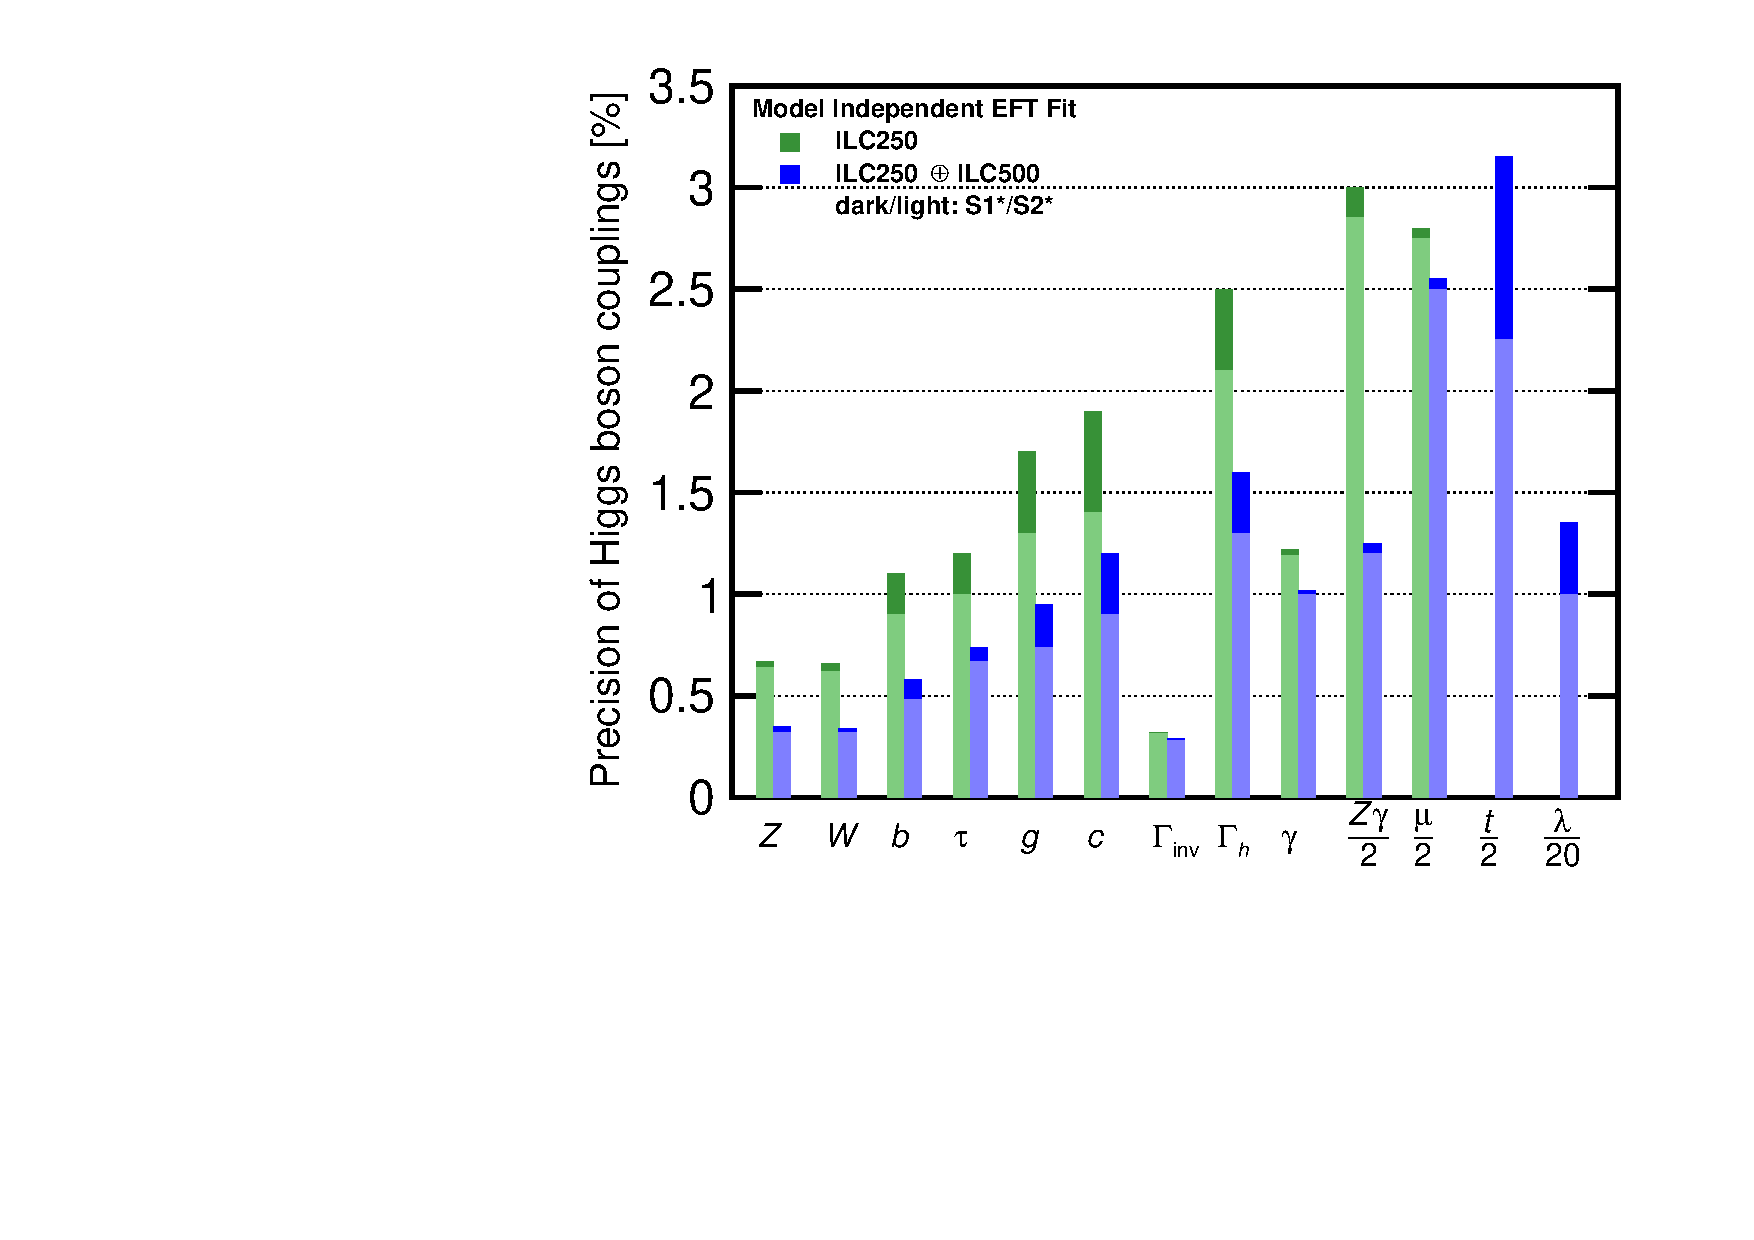
\includegraphics[width=0.85\hsize]{chapters/figures/ModelindepSummary.pdf}
\caption{Projected Higgs boson coupling uncertainties for the ILC
  program at 250~GeV and an energy upgrade to 500~GeV, using the
  highly model-independent analysis presented in \cite{Fujii:2017vwa}. This
  analysis makes use of  data on $\ee\to W^+W^-$ in addition to Higgs
  boson observables and also incorporates projected LHC results, as described
  in the text.  These
values correspond to the  scenario S1* in Table~\ref{tab:ILCLHC}.}
\label{fig:ILCmodelindep}
\end{center}
\end{figure}
%%%%%%%%%%%%%%%%%%%%%%%%%%%%%%%%%%%%%%%%%%%%%%%%%%%%%%%%%%%%%%
%%%%%%%%%%%%%%%%
\begin{figure}
\begin{center}
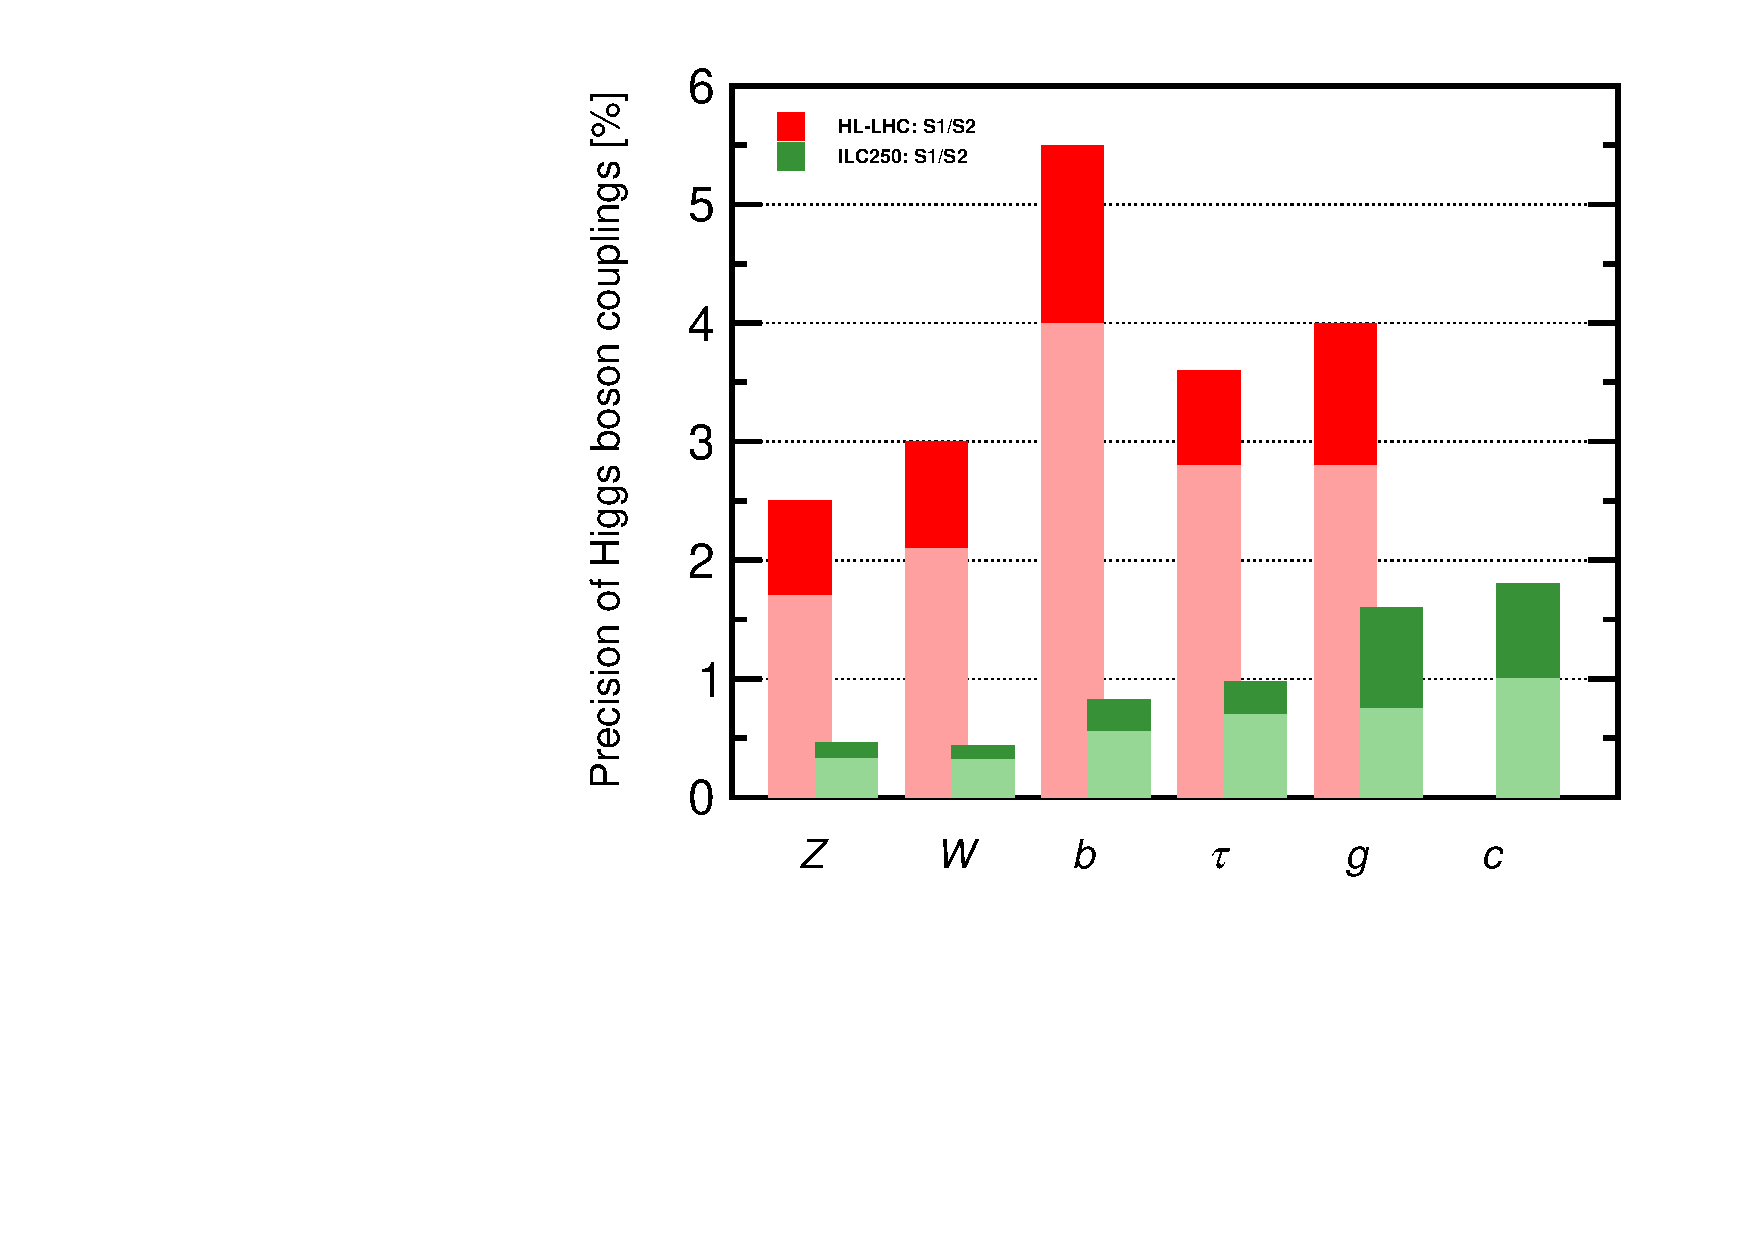
\includegraphics[width=0.85\hsize]{chapters/figures/ModeldepSummary.pdf}
\caption{Projected Higgs boson coupling uncertainties for the LHC and
  ILC
using the model-dependent assumptions appropriate to the LHC Higgs
coupling fit.   The
dark and light red bars represent the projections in the scenarios S1
and S2 presented in  \cite{YR}.    The dark and light green bars represent the
projections in the ILC scenarios S1 and S2 described in the
text.  The dark and light blue bars show the projections for scenarios S1 and S2
when
data from the 500~GeV run of the ILC is included.}
 \label{fig:ILCLHC}
\end{center}
\end{figure}
%%%%%%%%%%%%%%%%%%%%%%%%%%%%%%%%%%%%%%%%%%%%%%%%%%%%%%%%%%%%%%


The LHC S1 estimates do not assume such a model-independent framework.
Among the many model-dependent assumptions in the LHC  analyses, two are
particularly important. They  assume  that the Higgs boson has no decay
modes beyond those predicted in the SM, and they  assume that the Higgs
boson couplings to $WW$ and $ZZ$ are modified only by a rescaling.  In
the ILC EFT analysis, each of these these couplings depends on two
independent constants, called $\eta_{W,Z}$ and $\zeta_{W,Z}$ in
\cite{Barklow:2017suo}.   We can redo the ILC EFT analysis
adding these two assumptions, that is, assuming no
Beyond-Standard-Model decays and assuming $\zeta_{W} = \zeta_Z = 0$.
This gives the uncertainty estimates listed for ILC  in the column S1
in Table~\ref{tab:ILCLHC}.   We consider the comparison of the S1
uncertainties the most direct comparison of the capabilities of  LHC
alone with results of adding the ILC dataset. 
  We emphasize that the S1 analysis is 
simply a recast of the S1* estimates; the ILC inputs are based just 
as firmly in our full-simulation results.

%%%%%%%%%%%%%%%%%%%%%%%%%%%%%%%%%%%%%%%%%%%%5
\begin{table}[!htbp]
\begin{center}
\begin{tabular}{lccccc}
   coupling     &  current  &    S1*     &     S1     &    S2*   &   S2   \\ \hline 
$hZZ$ - LHC  &     11.      &        &       2.5   &        &  1.7 \\ 
\phantom{$hZZ$} - ILC 250 &      &   0.67  &  0.46   &   0.64   &  0.36 \\ 
\phantom{$hZZ$} - ILC 500&      &   0.35  &  0.20  &  0.32   & 0.18 \\ 
 \hline 
$hWW$ - LHC  &    15.       &        &    3.0     &        &  2.1 \\ 
\phantom{$hWW$} - ILC 250 &      &   0.66 &  0.44   &   0.62  &  0.36 \\ 
 \phantom{$hWW$} - ILC 500 &      &   0.34 &  0.19   &  0.32 & 0.18 \\ 
   \hline 
$hbb$ - LHC  &    29.       &        &          5.5   &        & 4.0 \\ 
\phantom{$hbb$} - ILC 250 &      &  1.1  & 0.83   &   0.90   &  0.68 \\ 
\phantom{$hbb$} - ILC 500 &      &  0.58  & 0.42   &  0.48  &  0.36 \\ 
 \hline 
$h\tau\tau$ - LHC  &    17.       &        &              3.6  &        & 2.8 \\ 
\phantom{$h\tau\tau$} - ILC 250 &      &  1.2  &  0.98   &   1.0  &  0.86 \\ 
\phantom{$h\tau\tau$} - ILC 500 &      &  0.74  &  0.63   &  0.67   & 0.59 \\ 
    \hline 
$hgg$ - LHC  &     15.      &        &            4.0   &        &
                2.8   \\ 
\phantom{$hgg$} - ILC 250 &      &  1.7  &  1.6   &   1.3   &  1.2 \\ 
 \phantom{$hgg$} - ILC 500 &      &  0.95  &  0.91   &  0.74  & 0.70 \\ 
\hline 
$hcc$ - LHC  &    -       &        &           -  &        &  - \\ 
\phantom{$hcc$} - ILC 250 &      &   1.9  &  1.8   &   1.4  &  1.3 \\ 
\phantom{$hcc$} - ILC 500 &      &  1.2  &  1.1   &   0.9  &  0.84 \\ 
    \hline 
$h\gamma\gamma$ - LHC  &    15.       &        &         3.6  &        & 2.8 \\ 
\phantom{$h\gamma\gamma$} - ILC 250  &      &   1.2  &  1.1  &   1.2   &  1.0\\ 
 \phantom{$h\gamma\gamma$} - ILC 500  &      &   1.0  &  0.99 &   1.0  &  0.97\\ 
\hline 
$h\mu\mu$ - LHC  &   70.        &        &     7.6  &        & 7.0 \\ 
\phantom{$h\mu\mu$} - ILC 250 &      &  5.6  &  5.6  &  5.5  &  5.5 \\ 
\phantom{$h\mu\mu$} - ILC 500 &      &  5.1  &  5.1  &  5.0  & 5.0\\ 
     \hline 
$htt$ - LHC  &   14.        &        &           5.5   &        &  3.6
  \\  
  \phantom{$htt$} - ILC 250  &        &   -     &     5.5    &  -   & 3.6
\\ 
\phantom{$htt$} - ILC 500  &        &    6.3    &     4.1     &    4.5   & 2.8
\\ 
\hline 
$hhh$ - LHC  &         &        &  80  &        &     60
  \\  
 \phantom{$hhh$} - ILC 500  &        &  -    &    80     &  -   & 60
\\ 
 \phantom{$hhh$} - ILC 500  &        &    27  &    27      &   20  & 20
\\ 
\hline \hline
$\Gamma_{tot}$ - ILC 250 &  &   2.5   &   1.3    &    2.1   & 1.1   \\ 
\phantom{$\Gamma_{tot}$} - ILC 500 & & 1.6 & 0.69 & 1.3  &  0.59  \\  \hline
$\Gamma_{inv}$ - ILC 250 &  &   0.32   &    -     &   0.32   &   -  \\ 
\phantom{$\Gamma_{inv}$} - ILC 500 & & 0.29 &  - & 0.28  & - \\  \hline
\end{tabular}
\end{center}
\caption{ \label{tab:ILCLHC}   Projected uncertainties in the Higgs
  boson couplings for LHC and for   and for ILC at 250~GeV, with
  precision LHC input, in various scenarios.   All values
  are given in percent (\%). The values labeled ``current'' are taken
  from Table 8 of the CMS publication \cite{Sirunyan:2018koj}.   The LHC S1 and
  S2 values are taken from \cite{YR}. The ILC scenarios are as
  described in this paper.  We also include our S1* and S1 projections
including the full ILC data set  with running at 250~GeV and 500~GeV. The ILC at 250~GeV only does not have direct sensitivity to the $htt$ and $hhh$ couplings; thus no  model-independent  values are given in these lines. The
  bottom lines give, for reference, the projected uncertainties in the
  Higgs boson total width and the 95\% confidence limits on the Higgs boson invisible width.  One should remember that one of the assumptions in the model-dependent S1/S2 fits is that the Higgs boson has no invisible or other exotic decay models.  We believe that the comparison of the S1
  values  gives the sharpest comparison between the capabilities of LHC
  alone and the capabilities after adding the ILC measurements. }
\end{table}

We have also attempted to produce a set of S2 estimates for the ILC.
These, by construction, go beyond our current understanding.  But it
has been true for electron colliders, just as for hadron colliders,
that actual experience in operating the experiments and working with
the 
data has led  to results that have exceeded the design levels of
performance.  To estimate the possible improvement, 
we have looked for elements in our work that 
are conservatively estimated and for which more detailed effort
making use of actual experience could produce a substantial
improvement.  Most of the improvement factors that we incorporate here
have already been estimated in 
preliminary ILD and SiD analyses.   There is also 
headroom in the ILC design for a possible
increase in luminosity (for example, by improving the tolerances in
the damping rings), but this is not included in our estimates.
  Using the more 
optimistic values as inputs to our 
model-independent analysis, we find the
uncertainties in the column S2*.  Applying also the model-dependent
assumptions
 listed above, we find the uncertainties shown in
 the column S2. 


Figures~\ref{fig:ILCmodelindep} and \ref{fig:ILCLHC}  illustrate the
capabilities of the ILC and the comparison of the ILC and LHC
projections.  Figure~\ref{fig:ILCmodelindep} shows the uncertainty
projections for the 250~GeV stage of the ILC, in the highly
model-independent framework S1*.  In the figure, these results are
compared to results obtained in the same framework with the addition
of data from an energy upgrade to 500~GeV.   This justifies the
statement made above that deviations from the SM seen at the 250~GeV
stage of the ILC can be confirmed with an independent data set after
the upgrade to higher energy.   Figure~\ref{fig:ILCLHC} shows the
comparison of the ILC projections in the S1 and S2 scenarios to the 
projections given for the S1 and S2 HL-LHC scenarios given in
\cite{YR}.  
Note that, while the improvement from the S1 to S2 scenarios is a
matter of conjecture, the improvement from the 250~GeV to the 500~GeV
values is based on completed full-simulation studies.
